\chapter{Code-mixing in the adjective-modified noun phrase}\label{NP}

This chapter investigates insertional code-mixing in noun phrases with adjective modifiers. In this syntactic context, the speaker may insert an attributive adjective from one contact language into a noun phrase headed by a noun from the other contact language. Alternatively, she can insert a nominal constituent that comprises a noun and an attributive adjective into a sentence framed by the other language. Hence, two patterns of code-mixing in this context are distinguished: the switch may be placed within the modified noun phrase or at the nominal constituent's boundary. Insertions of both nouns and nominal constituents, with and without modifiers, are well documented in the literature. For example, already \citet{poplack-sometimes-1980} offered empirical evidence suggesting that ``nouns and noun phrases are frequently switched'' (p. 604). Being ubiquitous in corpora of bilingual speech, nouns, nominal constituents and fully-fledged noun phrases have been the focus of extensive research along various lines \citep[e.g.,][]{sankoff-et-al-1990,poplack-meechan-1995, cantone-macswan,parafita-couto-et-al}.

The aim of this chapter is threefold: First, the chapter sets out to investigate patterns of code-mixing in the modified noun phrase in Russian-German bilingual sentences. Second, it aims to construct and assess a statistical model which predicts, by using phrase frequency and noun frequency as predictive factors, the variation in the way Russian-German bilinguals code-switch in the examined syntactic context. Third, the chapter explores the potential of usage-based explanations for code-mixing patterns in the noun phrase domain and thus contributes to clarify the ongoing discussion on the nature of adjective-noun insertions.

\begin{sloppypar}
To set the stage for the analysis, I first review the existing research on code-mixed nouns and nominal constituents, including adjective-modified noun phrases, and examine the issue of their status and nature as addressed by the major approaches. In section two, I outline the main features of adjective-noun combinations in German and Russian. The third section entails an analysis of Russian-German code-mixing in the context of the noun phrase modified by the attributive adjective. The fourth section introduces the main hypotheses underlying this chapter and investigates the factors suspected of regulating the variation in the scrutinised code-mixing patterns: switching within the adjective-modified nominal constituent and switching at its boundary. In the subsequent section, I present and assess the statistical model which predicts this variation. The final section entails a summary and a discussion of the main findings of the current study.
\end{sloppypar}

\section{Insertion of nouns and nominal constituents in bilingual speech}
\subsection{Noun insertion}\label{noun-insertion}
In language contact, nouns are involved in borrowing and in code-mixing more frequently than other word classes. Linguists who approach borrowing from a historical perspective \citep{whitney-1881, moravcsik, thomason-kaufman, matras2009} place nouns on top of borrowability hierarchies. Numerous studies of code-mixing show at the same time that noun insertion is the most frequent pattern of code-mixing. For instance, using multilingual data from the Gambia, \citet[112, 107]{haust-codeswitching-1995} finds that in her Mandinka-Wolof-English corpus, nouns constitute 55.8 per cent of all lexical morphemes inserted and integrated into the matrix language (327 of 586 tokens) and 66.5 per cent of all bare insertions (141 of 212 tokens). Researchers who regard noun insertion as borrowing \citep{poplack-etal-1988, sankoff-et-al-1990, van-hout-muysken, muysken-bilingual-2000}\footnote{It should be noted that \citet{muysken-bilingual-2000} acknowledges the equivocal status of single word insertion; he contends, ``Lexical borrowing has been associated with insertional code-mixing, and not without reason. Nouns are the class of elements borrowed par excellence and also the prime example of insertion under categorical equivalence'' (p. 75).} 
also report that bilingual speakers borrow nouns extremely often, even if, on certain occasions, noun insertions can count as switches (cf. Chapter \ref{CM-borrowing}). \citet[99--100]{treffers-daller-mixing-1994} demonstrates by using bilingual French-Dutch data that nouns constitute the greater part of single word switches (borrowings) in her Brussels corpus. She finds that French nouns encompass 58.4 per cent of overall French single word switches in Brussels Dutch, whereas Dutch nouns cover only 23.9 per cent of Dutch single word switches in French. (In fact, inserted Dutch nouns lie just behind inserted Dutch interjections with regard to both their token and type frequencies.) In total, noun switches still clearly dominate single word switches in the corpus. In conjunction with this, the question arises why nouns occupy such a prominent position in code-mixing and in the diachronic process of borrowing. 

One reason why nouns exhibit such a high degree of borrowability is their semantic nature. According to \citet{van-hout-muysken}, nouns, as prototypical content words, are borrowed because unlike function words they ``have a clear link to cultural content and the latter do not'' (p. 42). Moreover, nouns are notably prone to being selected in code-mixing because their meanings are highly specific \citep{backus-two-1996,backus-2001,field-2002}. \citet[115--131]{backus-two-1996} proposes a specificity continuum, with one pole formed by proper nouns and the other pole formed by schematic, or abstract, units. One of intermediate categories includes words denoting very specific objects. \citet[116]{backus-two-1996} defines these words as names for those concepts for which no other terms are available; these words are often referred to as cultural borrowings \citep[cf.][165]{myers-scotton-duelling-1993}. If we consider the word classes to which most proper names and cultural borrowings belong, we will state that most of them are nouns.\footnote{\citet{backus-two-1996} states that ``Especially in early stages of contact many single EL content words are names of some sort, such as place names and personal names, but also less obvious cases'' (p. 116).} A structural property of nouns that makes them highly borrowable is their high syntagmatic freedom \citep{backus-13}, which means that nouns are less bound to other words in the sentence and can thus be inserted in any sentence configuration. In language contact, especially in situations of intensive contact, the semantic and structural factors apparently interplay \citep[cf.][]{van-hout-muysken}.

Nouns can be inserted into virtually all possible configurations of the noun phrase. Louis Boumans (\citeyear[221]{boumans-syntax-1998}) characterises noun insertion as an unconstrained process. In his 1998 monograph \textit{\citetitle{boumans-syntax-1998}} he offers a detailed account of patterns in which Dutch nouns appear in the context of Moroccan Arabic. He describes various types of noun determination (p. 181--191, 211--214) and modification (p. 196--198, 200--205). In the latter case, he shows that inserted Dutch nouns can be modified by prepositional adjuncts and interrogative forms, but noun modification by Moroccan-Arabic adjectives is limited to few ``atypical'' instances \citep[200--201]{boumans-syntax-1998}. Furthermore, as nouns can subcategorise for complements in both Moroccan Arabic and Dutch, inserted Dutch nouns sometimes take Moroccan-Arabic prepositional and clausal complements. Unfortunately, \citet{boumans-syntax-1998} provides little or no information about the distribution of the various structures in the corpus.
Alongside single nouns, insertion of nominal constituents from another language is also commonplace in bilingual speech involving various language pairs. To this, I turn in the following section.

\subsection{Insertion of nominal constituents}{\label{nominal-constituents}}
Noun phrase insertions are commonplace in mixed clauses as well, although they are not as frequent as insertions of single nouns \citep[cf.][]{poplack-sometimes-1980}. For example, \citet[205]{treffers-daller-mixing-1994} observes that noun phrases make up 41.3 per cent of full-constituent switches in her French-Dutch data from Brussels. \citet[165]{haust-codeswitching-1995} also reports that noun phrases comprise the most frequent type of constituent insertion in her Gambian corpus: 79 noun phrases make up 47.9 per cent of 165 constituent insertions observed. Although such general quantitative data are not rare in studies of code-mixing, researchers often provide little or no information on the distribution of noun phrases varying in their structure. However, it is interesting to know what types of noun phrase modifiers and complements are more or less common in code-mixing and why. The aforementioned monograph by \citet{boumans-syntax-1998} represents an exception to this tendency insofar as it provides a comprehensive account of syntactic structures involved in Moroccan Arabic-Dutch code-mixing. Let us consider some of the findings regarding noun phrase insertion in greater detail. 

\citet{boumans-syntax-1998} shows that Dutch noun phrases inserted into Moroccan Arabic can be simple, such as \textit{het vermogen} `the capacity' in ({\ref{ex:4:1a}}), or expanded. The latter may contain a prepositional complement or an attributive adjective, as illustrated in (\ref{ex:4:1b}) and (\ref{ex:4:1c}).

\ea
Moroccan Arabic-Dutch \citep[212, 199, 212]{boumans-syntax-1998}\\

\ea{\label{ex:4:1a}}
\gll ʕend-i \textit{het vermogen} baš n.. eh ne-tbeʕ \textit{chemie}\\
    at-\textsc{1sg} \textsc{def.n} capacity \textsc{comp} 1-er 1-follow chemistry(Fr)\\
\glt `I have the capacity to study chemistry.'

\ex{\label{ex:4:1b}}
\gll kayn-in \textit{daar-voor} \textit{verklaring-en}\\
	\textsc{exist-pl} there-for explanation-\textsc{pl}\\
\glt `There are explanations for that.' 

\ex{\label{ex:4:1c}}
\gll ila bġi-tu t-reyyḥ-u ʕend-i, t-šerb-u l-atay u t-neʕs-u u te-mši-w eh \textit{de} \textit{volgend-e} \textit{dag} t-zid-u!\\
	if want-\textsc{2pl} 2-rest-\textsc{pl} at-\textsc{1sg} 2-drink-\textsc{pl} \textsc{def}-tea and 2-sleep-\textsc{pl} and 2-go-\textsc{pl} er the next-\textsc{agr} day 2-go.on-\textsc{pl}\\
\glt `If you (\textsc{pl}) want to stay at my place, you drink tea, you sleep, and you leave er the next day you go on.'
\z
\z

\noindent Fully-fledged Dutch noun phrases inserted into Moroccan-Arabic clauses are considerably less frequent than inserted nouns \citep[cf.][210]{boumans-syntax-1998}. Particularly insertion of expanded Dutch noun phrases is low in number. For example, the noun phrase with a prepositional complement and the noun phrase modified by a relative clause appear only twice each in the Moroccan-Arabic discourse in Boumans's data. In contrast, inserted Dutch nouns, as mentioned in (\ref{noun-insertion}), are freely modified ``by means of [Moroccan-Arabic] possessive constructions, adjunct or complement PPs, and relative clauses'' \citep[201]{boumans-syntax-1998}. Expanded Dutch nominal constituents, just like Dutch single nouns, often follow  Moroccan-Arabic determiners, as shown in  (\ref{ex:4:2a}), where the inserted Dutch noun \textit{nadeel} `disadvantage' follows the Moroccan-Arabic indefinite determiner \textit{ši} and is modified by the Dutch prepositional adjunct \textit{voor de universiteit} `for the university'.

\ea
Moroccan Arabic-Dutch \citep[198, 192]{boumans-syntax-1998}\\

\ea{\label{ex:4:2a}}
\gll u hadak š-ši y-kun \textit{nadeel} \textit{voor} \textit{de} \textit{universiteit}?\\
	and \textsc{dem} \textsc{def-indef}  3-be disadvantage for the university\\
\glt `And this will be a disadvantage for the university?'

\ex{\label{ex:4:2b}}
\gll {ʕla xaṭer} ʕend-ek ši  beʕḍ l-h.. \textit{handeling-en} \textit{die} \textit{je} {\textit{doet} (..)}\\
	because at-\textsc{2sg} \textsc{indef} part \textsc{def}-h.. action-\textsc{pl} that you do\\
\glt `Because you have some .. some actions that you do.'
\z
\z

\noindent Example (\ref{ex:4:2b}) illustrates the use of the Moroccan-Arabic definite article \textit{l-} with a Dutch nominal constituent, which consists here of the Dutch noun \textit{handelingen} `actions' and the modifying relative clause \textit{die je doet} `that you do'.\footnote{We can analyse the utterance in (\ref{ex:4:2b}) as an instance of revision: the speaker interrupts the utterance just before the switching site, i.e., at the beginning of the switched noun, so that the restart does not contain the Moroccan-Arabic determiner any more. It should be noted however that the same speaker produces smooth switches involving the Moroccan-Arabic prefix \textit{l-} as well \citep[cf.][185]{boumans-syntax-1998}.} As such, switching the language between determiner and noun has been frequently reported for other bilingual situations. According to \citet[604]{poplack-sometimes-1980}, this is a favourable locus for code-switching in her Spanish-English data. We can conclude from Boumans's analysis that insertion of fully-fledged Dutch noun phrases is less frequent than insertion of nominal constituents after Moroccan-Arabic determiners.

Noun-adjective combinations represent the most commonly inserted nominal constituents in Boumans's data \citep[cf.][203--205]{boumans-syntax-1998}. These insertions have an internal Dutch structure: first, the order of adjective and noun is A N, which is the opposite of the Moroccan-Arabic order, and secondly, the adjective exhibits the agreement marker \textit{-e} -- for all forms except for the indefinite singular neuter -- as in (\ref{ex:4:3}) below: 

\ea
\label{ex:4:3}
Moroccan Arabic-Dutch \citep[204]{boumans-syntax-1998}\\
\gll walakin daba d-derri ġadi ye-dxel \textit{islamitisch-e} \textit{school}, škun ġadi ye-lqa\\
	but now \textsc{def}-child \textsc{fut} \textsc{3m}-enter Islamic-\textsc{agr} school who \textsc{fut} \textsc{3m}-meet\\
\glt `But now the child will go to an Islamic school, whom will he meet?'
\z

\noindent The adjective-noun combination \textit{islamitische school} `Islamic school' is inserted without a determiner, the omission of determiner results from either the determinerless use of the noun \textit{school} in Dutch, as in the collocations \textit{naar school gaan} `go to school' and \textit{met school beginnen} `start school', or the tendency in Moroccan Arabic to omit the definite article before foreign stems \citep[cf.][187]{boumans-syntax-1998}. The omission of determiner with Dutch adjective-noun insertions in Moroccan Arabic discourse is as common as with Dutch single nouns. Hence, \citet[205]{boumans-syntax-1998} states that inserted adjective-noun combinations behave just like inserted nouns. Another point that needs emphasis here is that, unlike Dutch attributive adjectives, Moroccan-Arabic adjectives are never used to modify single Dutch nouns in Moroccan-Arabic discourse (cf. \ref{noun-insertion} and \citealt[][201]{boumans-syntax-1998}). Furthermore, Boumans asserts that Dutch adjectives are generally infrequent in Moroccan-Arabic sentences, even in the predicative function. Possible explanations for this observation are a lack of congruence between Moroccan Arabic and Dutch in the category of adjective and a mismatch between the involved languages in the adjective-noun order. However, as I will show in the subsequent section, this is not always the case and inserted nouns may well be modified by attributive adjectives in the same language when the patterns of adjective modifications employed by the contact languages vary.

\subsection{Inserted adjective-noun combinations}
Extensive insertion of adjective-noun combinations is characteristic not only of Moroccan-Arabic-Dutch code-mixing, but of code-mixing in general. Numerous studies of code-mixing have shown that adjective-noun combinations from one language appear in the discourse of the other language on a regular basis, regardless of the adjective-noun order that both languages use. As illustrated below, adjective-noun combinations are inserted into sentences in the other language when both languages share the adjective-noun order. For instance:

\ea{\label{ex:4:4}}
Turkish-Dutch \citep[177]{backus-two-1996}\\
\gll {\dots} {cuma günü} \textit{vaste} \textit{dag} yani\\
    {} {Friday.day} fixed day so\\
\glt `\dots we always go on Friday, so' 
\ex{\label{ex:4:5}}
Croatian-English \citep[231]{hlavac-second-generation-2003}\\
\gll {\dots} to sam završi-o dva tjedn-a, \textit{so} {\dots} i tako sam dobi-o rezultat-e \textit{last} \textit{week} i {\dots}\\
	{} that be.\textsc{prs.1sg} finish-\textsc{ptcp.sg.m} two week-\textsc{gen.sg} so {} and so be.\textsc{prs.1sg} receive-\textsc{ptcp.sg.m}  result-\textsc{acc.pl} {} {} and {}\\
\glt `\dots I finished that two weeks ago, so \dots and so I received the results last week and \dots'
\ex{\label{ex:4:6}}
German (dialect)-Hungarian \citep[373]{szabo-language-2010}\\
\gll {\dots} ihr ha-t \textit{szociális} \textit{villany} ghab\\
	{} \textsc{2pl} have-\textsc{prs.2pl} social electricity[\textsc{nom.sg}] have.\textsc{ptcp}\\
\glt `\dots you have had a social benefit rate for electricity'
\z

\noindent The language constellations here -- Turkish-Dutch in (\ref{ex:4:4}), Croatian-English in (\ref{ex:4:5}), and German-Hungarian in (\ref{ex:4:6}) -- all use the A N order. The inserted noun-adjective combinations \textit{vaste dag} `fixed day' (in \ref{ex:4:4}), \textit{last week} (in \ref{ex:4:5}) and \textit{szociális villany} `social (benefit rate for) electricity' (in \ref{ex:4:6}) all exhibit the internal structure of the corresponding language: Dutch, English and Hungarian, respectively. That is, the Dutch adjective \textit{vast} takes the Dutch agreement marker \textit{-e} (cf. \ref{ex:4:3}), and the English adjective \textit{last} and the Hungarian adjective \textit{szociális} remain uninflected, as required by English and Hungarian, but neither Croatian nor German.

In contact situations with languages differing in the adjective-noun order, combinations of nouns and adjectives have also been reported among frequent insertions. This applies, for instance, to Moroccan Arabic-Dutch code-mixing discussed above (\sectref{nominal-constituents}). Another example is code-mixing between English and Welsh, since in Welsh, unlike in English, the head noun precedes the adjectival modifier \citep[cf.][260]{deuchar-congruence-2005}. In (\ref{ex:4:7}), the word combination \textit{main news} occurs in a Welsh sentence, the English adjective-noun order indicates that the internal structure of this nominal constituent is English.

\ea{\label{ex:4:7}}
Welsh-English \citep[261]{deuchar-congruence-2005}\\
\gll ar y \textit{main} \textit{news}, ar y \textit{news} oedd o\\
	on \textsc{det} {} {} on \textsc{det} {} be.\textsc{3s.imp} \textsc{pron.3s.m}\\
\glt `On the main news, it was on the news'
\z

An excellent source of further examples for this case is the (\citeyear{gardner-chloros-1991}) study by Penelope Gardner-Chloros. The author reports numerous insertions of nominal constituents containing adjectives in her French-Alsatian data from Strasbourg. Again, the involved languages contrast in the adjective-noun order, though not as categorically as English and Welsh. While attributive adjectives in Alsatian occupy the position preceding the head noun, the position of adjectives in French can vary: most attributive adjectives follow their head nouns, but a reasonably large group of adjectives occur pre-nominally. With regard to the adjective-noun order, both types of combinations are registered, even though combinations with the N A order seem to dominate all French noun-adjective insertions  \citep[cf.][141]{gardner-chloros-1991}. The presented data contain instances such as \textit{gouverneur militaire} `military governor', \textit{groupement alsatique} `Alsatian co-operative', \textit{portes} \textit{ouvertes} `open day', \textit{résidence secondaire} `holiday home', \textit{visites guidées} `guided tours', \textit{temps morts} `(cassette) blanks' (p. 148), but also combinations with the A N order, such as \textit{jeune homme} `young man' (p. 139). Interestingly, the bilingual speaker can realise the adjective at one point in French, as in \textit{toupie jaune} `yellow spinning top', and later in the same conversation in Alsatian, as in \textit{gäls toupie} `yellow spinning top' \citep[133]{gardner-chloros-1991}. The latter example illustrates the possibility of single French nouns to be modified by Alsatian adjectives, as in \textit{e kleini attention} `a little treat' (p. 120), \textit{wunderbari charcuterie} `wonderful charcuterie' (p. 124) and  \textit{e klanni note} `a little note' (p. 140). It appears from this brief survey that despite the highly restricted congruence between Alsatian and French in the order of noun and its adjectival modifier, Alsatian-French bilingual speech exhibits considerable variability regarding code-mixing patterns in nominal constituents with attributive adjectives. These findings contrast strongly with those of \citet{boumans-syntax-1998} on code-mixing between Moroccan Arabic and Dutch, which also use differing adjective-noun orders. As such, single Dutch nouns, unlike single French nouns in Alsatian discourse, are not modified by Moroccan-Arabic attributive adjectives (cf. \ref{noun-insertion}). This comparison demonstrates that, although differing adjective-noun-order patterns may restrict adjectival modification of insertions by the other-language adjectives, as in the case of Moroccan-Arabic and Dutch code-mixing, they do not automatically rule out this possibility altogether. However, distributional properties of adjectival modification in bilingual sentences across various language pairs as well as different theoretical orientations have brought some scholars to conclude that adjective-noun combinations in the context of the other language pertain to the domain of  lexicon, and others to suggest that insertion of nominal constituents operates in the domain of the grammar. The existing approaches to adjective-noun insertions are detailed in the following section. I first discuss their status as lexical or grammatical forms, and then turn to explanations of their occurrence in bilingual speech.

\subsubsection{Status of inserted adjective-noun combinations}
The status of inserted adjective-noun combinations is the focus of much current controversy: while some scholars consider them pertinent to the lexicon, others regard them as inserted nominal constituents and thus a matter of grammar. In a detailed study on Tamil-English code-mixing, \citet{sankoff-et-al-1990} analyse English adjective-noun combinations in Tamil sentences, such as in (\ref{ex:4:8}), as lexical borrowings.

\ea{\label{ex:4:8}}
Tamil-English \citep[96]{sankoff-et-al-1990}\\
\gll \textit{Religion}-uDaya \textit{main purpose} vantu oru \textit{supernatural} \textit{being}-la oru \textit{belief} \textit{create} paNNaratu.\\
	\textcolor[rgb]{1,1,1}{Religion}-\textsc{gen} {} \textsc{ptcl} \textsc{det} {} \textcolor[rgb]{1,1,1}{being}-\textsc{loc} \textsc{det} {} {} do.\textsc{inf}\\
\glt `Religion's main purpose is to create a belief in a supernatural being.'
\z

\noindent They assume noun-adjective combinations, such as \textit{main purpose} and \textit{supernatural being}, to have the status of compound borrowings -- whether nonce, or established -- because ``the function words typical of English NPs \textit{never} co-occur with them'' \citep[80, emphasis in the original]{sankoff-et-al-1990}. Other compound nonce-borrowings include \textit{snide remarks}, \textit{serious subjects}, \textit{educational system}, \textit{slacks and blouses}, \textit{Government of India Scholarship}, \textit{Hindi songs}, \textit{Indian women}, \textit{arranged marriage} \citep[80, passim]{sankoff-et-al-1990}. This analysis is criticised by \citet[78--81]{muysken-bilingual-2000} for several reasons. His central argument against the nonce-borrowing analysis is that the borrowing process, for the most part, does not apply to multiword combinations at such a high rate as is the case with the material presented in \citet{sankoff-et-al-1990}. Nevertheless, Muysken agrees that ``complex'' nouns such as \textit{supernatural being} in (\ref{ex:4:8}) are borrowable per se, because they might have been lexicalised already in English (p. 79). His alternative  analysis assumes that these constructions are inserted NPs and thus a matter of syntax, rather than the lexicon.

A further relevant study into the nature and status of inserted nominal constituents is \citet{poplack-meechan-1995}. In this study of Wolof-French code-mixing, the authors examine complex French nouns that occur in otherwise Wolof sentences. Among these nouns are instantiations of the French `N \textit{de} N' construction, such as \textit{langue de cuisine} `broken language' and \textit{conditions de vie} `living conditions' \citep[215]{poplack-meechan-1995}. In (\ref{ex:4:9a}), a French construction \textit{tête de liste} `head of the list' is followed by the post-nominal Wolof determiner \textit{bi}.

\ea Wolof-French \citep[215, 228]{poplack-meechan-1995}\\

\ea{\label{ex:4:9a}}
\gll fexeel ba nekk ci \textit{tête} \textit{de} \textit{liste} bi rek.\\
	try.\textsc{imp} until be \textsc{prep} head of list \textsc{def} \textsc{adv}\\
\glt `Try to be only at the head of the list.' 

\ex{\label{ex:4:9b}}
\gll fokk naa moom moo la \textit{envoyer}-woon \textit{lettre} bi \textit{quoi}.\\
	think I him \textsc{foc}.he you send-\textsc{past} letter \textsc{def} what\\
\glt `I think it's him that had send you the letter eh.' 
\z

\z

\noindent \citet[215]{poplack-meechan-1995} report that `N \textit{de} N' constructions in Wolof sentences take the Wolof determiner \textit{bi}, just like single French nouns in Wolof discourse (as example \ref{ex:4:9b} with the noun \textit{lettre} `letter' demonstrates). Therefore, the authors regard the individual instances of the `N \textit{de} N' construction as loanwords. In doing so, they adopt the view outlined in \citet{sankoff-et-al-1990}, but introduce another diagnostic feature of (nonce-)borrowing: the semantic nature of a word sequence. The authors assert that ``the `N \textit{de} N' constructions virtually all consist of frozen or idiomatic expressions functioning as compounds'' (p. 215). Hence, the lexicalised nature of the examined sequences is a further argument in favour of their analysis as borrowings. 

As regards Dutch adjective-noun combinations occurring in Moroccan-Arabic sentences (cf. \sectref{nominal-constituents}) and French noun-adjective combinations in Alsatian discourse, these combinations are reminiscent of the French `N \textit{de} N' constructions in the Wolof discourse and, following Poplack and Meechan's structural and semantic criteria, count as borrowings. As mentioned above, in  \citeauthor{muysken-bilingual-2000}'s (\citeyear{muysken-bilingual-2000}) view, these combinations of nouns and adjectives are inserted NPs. An intermediate position in this controversy is taken, for example, by \citet[141]{gardner-chloros-1991}, who introduces the category of “lexical switches”, encompassing the noun-adjective combinations under discussion.

Another possibility to analyse adjective-noun combinations is to approach them from the Matrix Language Frame model proposed by \citet{myers-scotton-duelling-1993}. According to this model and its extensions (see Chapter \ref{CM} for further details), noun-adjective combinations in focus would be classified as ``EL islands'' as they are ``full constituents consisting only of Embedded Language morphemes occurring in a bilingual CP [Complementiser Phrase] that is otherwise framed by the Matrix Language'' \citep[139]{myers-scotton-contact-2002}. The internal structure of an embedded-language island corresponds to the norms of the language that provides the morphemes. For example, in (\ref{ex:4:7}), the adjective-noun combination \textit{main news} follows English norms, whereas the rest of the sentence is in Welsh \citep[cf.][261]{deuchar-congruence-2005}. We can assert that the examples of adjective-modified nouns quoted above as well as the aforementioned instances of the French `N \textit{de} N' construction are well-formed embedded-language islands. Whether these combinations are borrowed, or inserted, the question arises as to what factors determine the selection of the adjective modifying the inserted noun, or under what circumstances an attributive adjective comes from the same language as the inserted noun and when it comes from the other language.

\subsubsection{Explanations for inserting adjective-noun combinations}\label{explanations}
One of the first explanations for the insertion of adjective-noun combinations is offered through the Matrix Language Framework model, which treats these combinations as embedded-language islands. As outlined in \sectref{MLF}, \citet{myers-scotton-matching-1995} assert that an embedded-language island may occur if two languages lack congruence in one of three aspects of ``lemmas'', i.e., abstract entries in the mental lexicon that underlie lexemes. These aspects include semantic/pragmatic features, predicate-argument structure and realisation patterns. However, this view neither details which of the three aspects motivates the emergence of an embedded-language island in a given context, nor is it susceptible to an empirical verification. It is apparently this consideration that has lead some scholars to restrict their analyses of embedded-language islands to a specific type of congruence. For example, \citet{deuchar-congruence-2005} assumes that ``while the lack of semantic/pragmatic equivalence between lexemes in two languages may be an important cause of code-switching [which corresponds to code-mixing here] in the first place, it is considerations of grammatical rather than semantic congruence which determine whether or not a switch can take place'' (p. 258).\footnote{At the same time, \citet{deuchar-congruence-2005} mentions one of Wei's (2001) findings that incongruence in semantic/pragmatic features or predicate-argument structure can motivate occurrences of English embedded-language islands in otherwise Chinese discourse \citep[quoted in][258]{deuchar-congruence-2005}.} In case of nominal constituents containing an attributive adjective, congruence applies to word order within the constituent, or, in Myers-Scotton's terms, to morphological realisation patterns. As discussed above, word-order non-equivalence may account for the occurrence of embedded-language islands consisting of a noun and an attributive adjective in such language pairs as Moroccan Arabic-Dutch, Welsh-English, and possibly Alsatian-French. Nonetheless, this explanation would not hold for inserted adjective-noun combinations in language pairs with an identical noun-adjective order, namely Turkish-Dutch, Croatian-English, German-Hungarian and Tamil-English.

\begin{sloppypar}
Another explanation of nominal constituent insertions at non-equivalence sites is adumbrated by \citet[215]{poplack-meechan-1995}. They assert that nominal constituents, such as the `N \textit{de} N' constructions, can be borrowed because they comprise ``frozen or idiomatic expressions''. This point recalls Backus (1996, 1999, 2003), who elaborates the idea that idiomatic expressions are one type of multimorphemic lexical units which are inserted into a matrix language clausal frame. The ``unit'' hypothesis, laid out in \sectref{unit-hypothesis}, predicts that every embedded-language island is a unit \citep[cf.][91]{backus-units-2003}. Backus defines as units such multimorphemic elements that exhibit irregular morphosyntax, non-compositional semantics or high frequency. A multimorphemic element distinguished by one of these characteristics is assumed to be stored in the mental lexicon as a whole. Its parts are welded together by the irregularity of its form or the frequency of co-occurrence. However, it is possible to hypothesise that bilingual corpora may contain embedded-language islands lacking these properties. When such sequences do not count as multimorphemic units, their occurrence in bilingual clauses would remain unexplained. An example of a multimorphemic sequence lacking the characteristics of a unit is the aforementioned French combination \textit{toupie jaune} `yellow spinning top', inserted into an Alsatian framing clause (remember that in further discourse the speaker realises the adjective in Alsatian, i.e., \textit{gäls toupie}, \citealt[133]{gardner-chloros-1991}). The French string is neither frequent in French, nor is its meaning non-compositional. Furthermore, adjective-noun order differences between French and Alsatian cannot be a valid explanation for the insertion of \textit{toupie jaune} as well (in view of the French adjective-noun insertions in the Alsatian discourse). Hence, the obvious way to examine the ``unit'' hypothesis is to test it statistically.
\end{sloppypar}

A distinction between fixed expressions and ad hoc produced strings underlies the analysis of Russian nominal constituents in Kazakh discourse in \citet[77--88]{muhamedowa-untersuchung-2006}. Although the author claims to have adopted Backus's approach, only expressions that originate from the Russian institutional language are considered fixed. Namely, multiword strings such as \textit{metodičeskij otdel} `curriculum and instruction department' (p. 77) and  \textit{ministerstvo lëgkoj promyšlennosti} `ministry of light industry' (p. 79) are analysed as fixed, whereas the strings \textit{staryj ploščad'} `old square'\footnote{It is worth noting that the adjective \textit{staryj} `old' lacks gender agreement with the feminine head noun \textit{ploščad'} `square' \citep[82]{muhamedowa-untersuchung-2006}.} in (\ref{ex:4:10}) and \textit{vysotnye doma} `high-rise houses' (p. 81) are regarded as ad hoc creations. 

\ea{\label{ex:4:10}}
Kazakh-Russian \citep[82]{muhamedowa-untersuchung-2006}\\
\gll anau \textit{televizor}-dan kör-gen šïğar-sïz-dar. ne-ler-i-n \textit{uže} anau \textit{star-yj} \textit{ploščad'}-tï ne-ler-di žönde-di, anau universitet ne qïl-dï.\\
	that {TV.set}-\textsc{abl} see-\textsc{perf} perhaps-\textsc{pol-2pl} thingummy-\textsc{pl-pos3-akk} already that old-\textsc{nom.sg.m} square[\textsc{nom.sg.f}]-\textsc{acc} thingummy-\textsc{pl-acc} improve-\textsc{3sg} that university thingummy do-\textsc{3}\\
\glt `Perhaps you have seen that on TV. They have renovated that Old Square and the thingummy already, and they did that thingummy at university.'
\z

\noindent However, the adjective-noun combination \textit{staryj ploščad'} `old square' in (\ref{ex:4:10}) is obviously a place name and could thus be a fixed routine in the speaker's idiolect and a lexical unit in her mental lexicon. This may be the case because place-names are unlikely to be produced compositionally on-line. As for the string \textit{vysotnye doma} `high-rise houses', it is a fairly regularly occurring collocation in Russian: 17\% of all occurrences of the adjective \textit{vysotnyj} `high-rise' in the Russian National Corpus comprise instances in which this adjective combines with the noun \textit{dom} `house'.\footnote{The adjective \textit{vysotnyj} `high-rise' co-occurs at a higher rate only with the noun \textit{zdanie} `building'.} Consequently, the string should be viewed as a  collocation and thus a lexical unit. We can conclude that Muhamedowa utilises register as an indicator of a string's fixedness. But classifying embedded-language noun-adjective combinations by virtue of register alone appears to be insufficient for determining the status of these combinations as lexical units. Furthermore, most of the examples in \citet[81--88]{muhamedowa-untersuchung-2006} can well be subsumed under the category of lexical unit. 

The final study to be discussed in this section is again the analysis of Dutch adjective-noun insertions in Moroccan Arabic by \citet{boumans-syntax-1998}. According to the author, in a situation in which embedded Dutch nouns are regularly modified by Dutch attributive adjectives but virtually never occur with Moroccan-Arabic adjectives, the selection of attributive adjectives, restricted by the noun being modified, results from ``specific ties that bind nouns and attributive adjectives from the same language'' (p. 220). By elaborating this point further, he provides support for Backus's (1996) conception: the ties between nouns and attributive adjectives are of collocational nature and are obviously not limited to idiomatic expressions \citep[cf.][386--387]{boumans-syntax-1998}. This consequence is extended to other multiword embedded-language islands. Existence of collocational ties can account not only for Dutch noun-adjective insertions in Moroccan Arabic, but also for fully-fledged phrases, like \textit{de volgende dag} `the following day' in (\ref{ex:4:1c}). As the definite determiner \textit{de} co-occurs with the string \textit{volgende dag} much more often than the indefinite determiner \textit{een}, we can assume that the string \textit{de volgende dag} is a unit, which is stored and selected as a whole in on-line production. \citet{boumans-syntax-1998} concludes the section on collocational ties by suggesting that ``[i]f the existence of collocational ties between lexical units in the mental lexicon accounts for the co-occurrence of EL [embedded-language] words, the total absence of such ties may perhaps explain the observed constraints on the co-occurrence of ML [matrix language] and EL [embedded-language] lexical items'' (p. 386--387). This means that an approach elucidating the emergence of embedded-language islands in bilingual speech has also the potential to clarify the intricacies of mixed constituents. Moreover, this idea provides a starting point for the subsequent study: in order to prove the existence of collocational ties, we need to compare inserted adjective-noun combinations with noun insertions modified by attributive adjectives from the matrix language.

To recapitulate, scholars suggest both structural and semantic explanations underlying embedded adjective-noun combinations in code-mixing. A structural approach considers incongruence between the involved languages in the realisation patterns of adjective-modified nominal constituents as a crucial factor \citep{myers-scotton-matching-1995, myers-scotton-contact-2002}. In other words, non-equivalence in the noun-adjective order can trigger the emergence of an embedded language island realised as an adjective-modified nominal constituent \citep{deuchar-congruence-2005}. However, this explanation will fail for language constellations with an identical adjective-noun order, like German and Russian. Some scholars \citep[e.g.,][]{poplack-meechan-1995} state that at least some embedded nominal constituents are idiomatic expressions. Although plausible at first sight, this explanation will not account for embedded adjective-noun combinations lacking non-compositional meanings. Finally, Backus (1996) and Boumans (1998) consider noun-adjective combinations multiword lexical units, even when their semantics is compositional. Frequently used combinations, whose meaning may be compositional, also gain unit status in this approach. \citet{boumans-syntax-1998} argues that it is collocational ties between a noun and an adjective that determine their insertion as a combination in code-mixing.  However, owing to a high variability observed in code-mixing, not every inserted adjective-noun combination would obviously qualify as a unit. Moreover, in order to obtain unequivocal evidence for the existence of collocational ties, it is insufficient to rely on code-mixing data alone; rather, examined collocations have to be investigated in both bilingual and monolingual speech. Therefore, following the report of the code-mixing patterns in the examined syntactic context as they occur in my corpus of Russian-German bilingual speech, I will analyse the adjectival modification of the obtained nouns in large monolingual corpora and will finally subject these results to statistical test. However, before turning to these issues, I will briefly introduce the patterns of adjectival modification in German and in Russian.

\section{Adjective-noun combinations in German and Russian}
In languages of the world, attributive adjectives may either precede or follow their head nouns. German and Russian employ both syntactic patterns for noun modification. However, the most common pattern is when attributive adjectives occur in the prenominal position and agree with their head nouns in gender, number and case (\citealt[1303]{rusgramm-tom1}; \citealt[232]{eisenberg-satz-1999}). For example:

\ea
\label{ex:4:11}
German \citep[1991]{ids-3-1997}\\
\textit{ein} \textit{klein-es} \textit{grün-es} \textit{Männchen}\\
	\textsc{art[nom.sg.n]} little-\textsc{nom.sg.n} green-\textsc{nom.sg.n} man(\textsc{n})[\textsc{nom.sg}]\\
\glt `a little green man'
\z

\noindent In (\ref{ex:4:11}), the adjectives \textit{kleines} `small' and \textit{grünes} `green' precede the noun \textit{Männchen} `little man'. Furthermore, congruence in number, gender and case is observed between the forms of the adjective, the noun and the indefinite article \textit{ein}. This pattern of modification is also prototypical of Russian, for instance: 

\ea
\label{ex:4:12}
Russian\\
\textit{malen'k-ij} \textit{zelën-yj} \textit{čeloveček}\\
	little-\textsc{nom.sg.m} green-\textsc{nom.sg.m} man[\textsc{nom.sg.m}]\\
\glt `a little green man'
\z

\noindent The attributive adjectives \textit{malen'kij} `small' and \textit{zelënyj} `green' in (\ref{ex:4:12}) precede the noun \textit{čeloveček} `little man' and agree with it in number, gender and case. 

At the same time, Russian and German adjectives may also follow the noun. Particularly in German, this pattern is restricted to special contexts and individual lexical items. German adjectives occupy the postnominal position in the following four cases: (i) adjectives are postposed as a result of topicalisation (i.e., split topicalisation), as in (\ref{ex:4:13a}); (ii) adjectives occur in apposition to nouns in names of products and dishes\footnote{The case of appositive adjectives is not limited to these contexts; apposition is traditionally characteristic of literary, poetic and folk-song texts \citep[cf.][1991]{ids-3-1997} and has recently expanded to press texts \citep{duerscheid-2002}. In the latter case, such adjectives as \textit{brutal}, \textit{light} `easy',  \textit{total} `sheer' often appear in postposition (e.g., \textit{Fußball brutal} `brutal football', \citealt[67]{duerscheid-2002}). However, the use of adjectives in these contexts is immaterial in the further analysis.}, as in (\ref{ex:4:13b}); and (iii) specific lexemes, such as \textit{bar} `cash' and \textit{pur} `pure', tend to follow their head nouns, as in (\ref{ex:4:13c})\footnote{This outline does not include the case of adjectival increments, also analysed as loose appositions \citep[654]{auer-increm}. For example, the postnominal adjectives \textit{bayrische} `Bavarian' and \textit{geschnitten} `cut' in the following instances are distinguished by an appositive relation to their head nouns: \textit{eine mode eine bayrische} `a fashion, a Bavarian one' (Schröder 1997, p. 103, quoted in \citealt[142]{schwitalla-2006}) and \textit{[...] und möhrchen brauch ich klein geschnitten} `and I need carrots, cut in small pieces' \citep[654]{auer-increm}.}.

\ea

\ea{\label{ex:4:13a}}
\citep[234]{eisenberg-satz-1999}\\
\gll \textit{Geld} \textit{hilf-t} \textit{dir} \textit{nur} \textit{gefälscht-es} \textit{weiter}\\
	money(\textsc{n})[\textsc{nom.sg}] help-\textsc{3sg} \textsc{dat.2sg} only forged-\textsc{nom.sg.n} \textsc{ptcl}\\
\glt `Money will help you, only if it is fake'

\ex{\label{ex:4:13b}}
\citep[64, 78]{duerscheid-2002}\\
\gll \textit{Whisky} \textit{pur}, \textit{Forelle} \textit{blau}, \textit{Schauma} \textit{mild}\\
	whisky(\textsc{m})[\textsc{sg}] straight, trout(\textsc{f})[\textsc{sg}] blue, Schauma(\textsc{n})[\textsc{sg}] mild\\
\glt `Straight whisky, blue trout, mild Schauma'

\ex{\label{ex:4:13c}}
(\citealt[350]{duden-2009}; \citealt[67]{duerscheid-2002})\\
\gll \textit{tausend} \textit{Euro} \textit{bar}, \textit{Natur} \textit{pur}\\
	thousand euro(\textsc{m})[\textsc{sg}] cash, Natur(\textsc{f})[\textsc{sg}] pur\\
\glt `A thousand euros in cash, pure Nature'
\z
\z

\noindent As is evident from the above examples, German postnominal adjectives inflect for gender, number and case when their head nouns are topicalised (cf. \ref{ex:4:13a}), whereas the postnominal adjectives \textit{bar} `cash' and \textit{pur} `pure' as well as adjectives in product names remain bare.

With regard to Russian, \citet[149]{zemskaja} reports that in the colloquial speech, attributive adjectives occur in the postnominal position more frequently than in the written language, for example: 

\ea
\label{ex:4:14}
\citep[152]{zemskaja}\\
\gll \textit{Prines-i} \textit{xleb-a} \textit{svež-ego}; \textit{A} \textit{gde} \textit{jubk-a} \textit{sinj-aja}?\\
	bring-\textsc{imp} bread-\textsc{gen.sg.m} fresh-\textsc{gen.sg.m} and where skirt-\textsc{nom.sg.f} blue-\textsc{nom.sg.f}\\
\glt `Bring some fresh bread; And where is the blue skirt?'
\z

\noindent \citet{zemskaja} asserts that the postposed adjectives \textit{svežego} `fresh' and \textit{sinjaja} `blue' in (\ref{ex:4:14}) do not carry a special information load and are thus devoid of prosodic emphasis \citep[cf.][208--212]{lapteva}. According to \citet{zemskaja}, prepositioned adjectives tend to carry information load and prosodic emphasis, particularly when the noun phrase appears in the clause-initial position, as in (\ref{ex:4:15}).

\ea
\label{ex:4:15}
\citep[153]{zemskaja}\\
\gll \textit{Krasiv-ye} \textit{cvet-y} \textit{ja} \textit{segodnja} \textit{kupi-l-a}\\
	beautiful-\textsc{acc.pl.m} flower-\textsc{acc.pl.m} \textsc{nom.1sg} today buy-\textsc{pst-sg.f}\\
\glt `What beautiful flowers have I bought today!'
\z

\noindent However, \citet[208, 211, 221--222]{lapteva} considers both templates as functionally equal variants.

A further criterion for a syntactic description of Russian attributive adjectives is the distance between adjectives and their noun heads. Unlike in German, where attributive adjectives occupy only the positions immediately adjacent to their head nouns, adjectives in Russian may take positions distant from their noun heads. For instance:

\ea
\ea{\label{ex:4:16a}}
\citep[165]{miller-weinert}\\
\gll \textit{interesn-uju} \textit{prines-i} \textit{mne} \textit{knig-u}\\
	interesting-\textsc{acc.sg.f} bring-\textsc{imp} \textsc{dat.1sg} book-\textsc{acc.sg.f}\\
\glt `Bring me an interesting book.'

\ex
\label{ex:4:16b}
\citep[213]{lapteva}\\
\gll \textit{Pojd-u} \textit{prines-u} \textit{stul'čik} \textit{sebe} \textit{malen'k-ij}\\
	go[\textsc{perf.prs}]-\textsc{1sg} bring[\textsc{pfv.prs}]-\textsc{1sg} little.chair[\textsc{acc.sg.m}] \textsc{refl.dat} small-\textsc{acc.sg.m}\\
\glt `I'll go and get myself a small chair.'
\z
\z

\noindent While the adjective of the “split” noun-phrase \textit{interesnuju -- knigu} `interesting book' in (\ref{ex:4:16a}) appears in the prenominal position, the adjective \textit{malen'kij} `small' in (\ref{ex:4:16b}) occurs in the postnominal position. The distant prenominal position of the adjective \textit{interesnuju} `interesting' in (\ref{ex:4:16a}) is explained by a special information purpose, namely highlighting the adjective \citep[153]{zemskaja}. \citet{miller-weinert} state that distant prenominal adjectives ``are equal to or more important than the noun with respect to information load'' (p. 167). As regards postnominal adjectives, as in (\ref{ex:4:16b}), \citet[213]{lapteva}  and \citet[153]{zemskaja} describe one of their functions as elaboration. In this function, the adjectives are weak semantically and prosodically. Although the question of how syntactic configurations of attributive adjectives combine with intonation patterns to express various discursive meanings is of theoretical and practical interest, it is beyond the scope of this work and will not be discussed further.

The subsequent analysis of Russian-German bilingual data requires us to distinguish between the aforementioned case of distant postnominal adjectives, as in (\ref{ex:4:16b}), and the case of adjectival increments, as in (\ref{ex:4:17}).

\ea
\label{ex:4:17}
\citep[155]{zemskaja}\\
\gll \textit{Ona} \textit{zvoni-l-a} \textit{tët-e} \textit{Oksan-e}  \textit{čtoby} \textit{ona\dots} \textit{kupi-l-a} \textit{tort} \textit{èt-ot} \textit{sam-yj}, \textit{s} \textit{proslojk-ami}, \textit{vafel'n-yj}\\
	\textsc{nom.3.sg.f} call-\textsc{pst-sg.f} aunt-\textsc{dat.sg.f} Oksana-\textsc{dat.sg.f} so.that \textsc{nom.3.sg.f} buy-\textsc{pst-sg.f} cake[\textsc{acc.sg.m}] that-\textsc{acc.sg.m} very-\textsc{acc.sg.m} with layer-\textsc{instr.sg.f} wafery-\textsc{acc.sg.m}\\
\glt `She called aunt Oksana to ask her to buy that cake, with layers, a wafer one.'
\z

\noindent The prepositional phrase \textit{s proslojkami} `with layers' and the adjective \textit{vafel'nyj} `wafery' are placed at the end of the utterance, after the word \textit{samyj}, which is marked by a falling tone. According to \citet[155--156]{zemskaja}, the function of these structures is elaboration. The author discusses them in conjunction with the principle of ``associative adjoinment'', which enables the speaker to add any additional detail to the end of the utterance. Nonetheless, she is silent about the difference between distant postnominal adjectives, as in (\ref{ex:4:16b}), and adjectival increments, such as \textit{vafel'nyj} `wafery' in (\ref{ex:4:17}). The morphological criterion, which is adopted to distinguish postnominal adjectives from adjectival increments in German (recall that German postnominal adjectives in the case of split topicalisation are inflected for gender, number and case, whereas adjectival increments, which are in apposition to their head nouns, are uninflected, see footnote 8), does not apply to Russian adjectives in the postnominal position: both types of adjectives inflect for gender, number and case. On formal grounds, I regard as increments only those postposed adjectives which are produced after words marked by the falling terminal tone. Being clause-peripheral elements, adjectival increments are irrelevant to insertional code-mixing, and will thus not be considered further below. 

The last group of adjectives that need to be discussed in this outline are adjectives for which postposition is the only possible option. The use of such adjectives in Russian is restricted to two cases: (i) adjectives as part of classification terms and product names \citep[203]{rusgramm-tom2}\footnote{\citet{rijkhoff} uses the term ``classifying modifier'' to refer to this case.}, as in (\ref{ex:4:18a}), and (ii) morphologically unintegrated borrowings \citep[556]{rusgramm-tom1}, as in (\ref{ex:4:18b}). 

\ea
\ea{\label{ex:4:18a}}
\citep[203]{rusgramm-tom2}\\
\gll \textit{šalfej} \textit{lekarstvenn-yj}, \textit{šalfej} \textit{lugov-oj}; \textit{marmelad} \textit{jabločn-yj}, \textit{šokolad} \textit{soev-yj}\\
	sage[\textsc{nom.sg.m}] gardenly-\textsc{nom.sg.m} sage[\textsc{nom.sg.m}] meadow-\textsc{nom.sg.m} gumdrop[\textsc{nom.sg.m}] apple-\textsc{nom.sg.m} chocolate[\textsc{nom.sg.m}] soya-\textsc{nom.sg.m}\\
\glt `garden sage (\textit{salvia officinalis}), meadow sage (\textit{salvia pratensis}); apple gumdrop, soya chocolate'

\ex{\label{ex:4:18b}}
\citep[540]{rusgramm-tom1}\\
\gll \textit{cvet} \textit{bordo}, \textit{brjuk-i} \textit{klëš}, \textit{jubk-a} \textit{plisse}\\
	colour[\textsc{nom.sg.m}] claret trouser-\textsc{nom.pl.m} bell-bottom skirt-\textsc{nom.sg.f} plissé\\
\glt `a claret colour, bell-bottom trousers, a plissé skirt'
\z
\z

\noindent Interestingly, the morphologically non-integrated loans in (\ref{ex:4:18b}) \textit{bordo} `claret', \textit{klëš} `bell-bottom' and \textit{plisse} `plissé' have well-integrated counterparts: \textit{bordovyj}, \textit{klešënyj}\slash\textit{rasklešënnyj} and \textit{plessirovannyj}. These morphologically integrated loans, which are common in the Russian colloquial speech, may appear in the pre- or postnominal position,  as in \textit{bordovyj cvet} `the claret colour', \textit{klešënye brjuki} `bell-bottom trousers' and \textit{plessirovannaja jubka} `a plissé skirt'.

As follows from the overview of the syntactic configurations involving attributive adjectives in German and Russian, Russian exhibits a greater number of patterns for noun modification by adjectives than German. Beyond the few lexical restrictions, pragmatics seems to be the only factor that constrains the position of attributive adjectives in Russian. In contrast, German has one canonical position for attributive adjectives, i.e., the prenominal position. The postnominal position, in which adjectives are morphologically bare, is restricted to specific lexical items and classifying modifiers in special contexts. One of such contexts, the use of adjectives in product names, is found in both languages. Although inflection for the grammatical gender, number and case generally applies to adjectives in both German and Russian, it does not apply to German postnominal adjectives (with the exception of adjectives in split noun phrases with topicalised nouns) and certain borrowed adjectives in Russian. Despite the morphological non-equivalence in the inflection of adjectives observed in these two cases, the syntactic patterns, i.e., the adjacent preposition and the adjacent postposition, are identical in both languages. What is different between German and Russian syntactic patterns of modification is the possibility of distant modification, which exists only in Russian. In other words, only in Russian inflected attributive adjectives frequently occur detached from the head noun.

On the whole, modification by attributive adjectives exhibits similarities and differences in German and Russian: adjectives appear in both the pre- and postnominal position to modify their head nouns, but in German semantic and pragmatic constraints restrict the use of adjectives in the postnominal position more rigorously than in Russian, in which the postnominal position is commonplace in the colloquial speech. Considering this outline, we can predict that in insertional code-mixing, with Russian being the matrix language, Russian adjectives may pre- or post-modify German noun insertions, whereas inserted German adjective-noun combinations would follow the German order, such that the attributive adjective precedes the noun. In order to see whether this prediction is correct, we have to investigate these two types of insertion in the bilingual corpus.

\section{Adjective-noun combinations in the Russian-German bilingual corpus}
In my Russian-German bilingual corpus, the use of attributive adjectives in mixed sentences is observed to be limited to two cases: Firstly, combinations of German attributive adjectives and their German head nouns may be inserted into Russian sentences as embedded-language islands. Secondly, Russian adjectives may modify German nouns pre- and post-nominally. Instances of modification of Russian nouns by German adjectives are absent from the corpus, although German adjective insertions occur in the corpus as (subject) predicatives (see \citealt{deuchar-congruence-2005}, for a similar case in Welsh-English code-mixing).

\subsection{German adjective-noun combinations in Russian sentences}
German adjective-noun combinations appearing in Russian sentences can be analysed as instances of insertional code-mixing (see section 4.1.3). For example, the German noun phrase \textit{gebratene Nudeln} `fried noodles' in (\ref{ex:4:19}) is inserted into a Russian clause structure, namely, into a Russian prepositional phrase. 

\ea
\label{ex:4:19}
(LA-1205031A)\\
\gll ja xoč-u čë-nibud' s \textit{gebraten-e} \textit{nudel-n}\\ 
 \textsc{nom.1sg} want-\textsc{1sg} something with fried-\textsc{nom.pl} noodle-\textsc{pl}\\
\glt `I'd like something with fried noodles.'

\z

\noindent The internal structure of the inserted constituent \textit{gebratene Nudeln} is German: the adjective \textit{gebraten} `fried' agrees with its head noun in the number and takes the inflectional suffix \textit{-e}, which marks the nominative or the accusative case. The morphologically marked case deviates from the case projected by the preceding Russian preposition \textit{s} `with', namely, the instrumental case. This mismatch may be due to the absence of the instrumental case from the German case system.  However, since the prepositional phrase is a constituent of a higher level than the German noun phrase, the analysis of the German adjective-noun combination as an insertion holds despite the issue of the structural non-equivalence of the two systems.

Insertions of German nominal constituents containing attributive adjectives, which can be regarded as embedded-language islands from the viewpoint of the MLF model, are the most frequent case in the corpus: a total of 71 adjective-noun combinations were identified, which correspond to 65 lexical types. These extended noun phrases almost invariably lack German determiners. For example, the German inserted noun phrases \textit{chillige Familie} `chilly family' in (\ref{ex:4:20}) and  \textit{unbekanntes Gesicht} `unfamiliar face' in (\ref{ex:4:21}) would require indefinite articles \textit{eine} and \textit{ein}, respectively, when used in German sentences because they refer to countable indeterminate objects.

\ea
\label{ex:4:20}
(LS-110125J)\\
 \gll nee u menja \textit{chillig-e} \textit{familie}\\
 no with \textsc{gen.1sg} chilly-\textsc{nom.sg.f} family(\textsc{f})[\textsc{sg}]\\
\glt `No, I have a chilly family.'
\ex
\label{ex:4:21}
(LA-12022404A)\\
 \gll a mnje \textit{oh} \textit{nee} \textit{geh-t} \textit{nicht}; vidat' {to čto} u menja \textit{unbekannt-es} \textit{gesicht=}  da čto \textit{ich} \textit{komm-e} \textit{selten} \textit{oder} \textit{so=} \textit{ja}\\ 	
 but \textsc{dat.1sg} \textsc{ptcl} no go-\textsc{3sg} \textsc{neg} perhaps because with \textsc{gen.1sg} unfamiliar-\textsc{sg.n} face(\textsc{n})[\textsc{sg}] yes because \textsc{nom.1sg} come-\textsc{1sg} rarely or so yes\\ 
\glt `But (she says to) me, ``Oh no, that's impossible''; perhaps because my face is unfamiliar (to her), yes, because I come rarely or so, yes.'
\z

\noindent Even when the referents of the inserted noun phrases are definite objects, German articles are not used, for instance:

\ea
\label{ex:4:22}
(H-100712O)\\
\gll ei  smotr-i kak-ie igrušk-i; smotr-i \textit{na?}  gde \textit{klein-er} \textit{stern}?\\
 \textsc{ptcl} look-\textsc{imp.2sg} what-\textsc{nom.pl} toy-\textsc{nom.pl} look-\textsc{imp.2sg} \textsc{ptcl} where small-\textsc{sg.m} star(\textsc{m})[\textsc{sg}]\\
\glt `Ah, look, what (nice) toys! Hey, look, where is the small star?'
\ex
\label{ex:4:23}
(LV-12022404A)\\
\gll potom oni est' v \textit{historisch-es} \textit{seminar}\\
 then \textsc{nom.3pl} be[\textsc{prs}] in historical-\textsc{sg.n} department(\textsc{n})[\textsc{sg}]\\
\glt `Then there are some in the department of history.'
\ex
\label{ex:4:24}
(LA-1205034V)\\
 \gll vo-pervyx \textit{baltisch-e} \textit{länd-er-n}  otnosi-l-i-s' ne k rossi-i pri petr-e perv-om\\
 firstly Baltic-\textsc{pl} \textsc{pl}\textbackslash{}country-\textsc{pl-pl/dat} be.part-\textsc{pst-pl-refl} \textsc{neg} of Russia-\textsc{dat.sg.f} under Peter-\textsc{prep.sg.m} first-\textsc{prep.sg.m}\\
\glt `First of all, the Baltic countries were not part of Russia under Peter the First.'

\z

\noindent The noun phrases \textit{kleiner Stern} `small star' in (\ref{ex:4:22}), \textit{historisches Seminar} `historical department' in (\ref{ex:4:23}) and \textit{baltische Ländern}\footnote{The formative \textit {-n} is added to the noun \textit{Länder} apparently erroneously. We can interpret this form in at least two ways: the speaker either double marked the plural on the noun (cf. the standard singular \textit{Land} vs. the standard plural \textit{Länder}, or produced its dative plural form. The latter analysis seems yet rather implausible for two reasons: (i) the noun phrase, being the subject of the clause, should be assigned the nominative case and (ii) the adjective is not inflected for dative  (cf. \textit{baltischen Ländern}).} `Baltic countries' in (\ref{ex:4:24}) all lack definite articles, which would be mandatory in German clauses. Furthermore, the presence of the definite article before these noun phrases in German would require the use of inflectional suffixes of the ``weak'' declension, i.e., \textit{der klein-e Stern}, \textit{das historisch-e Seminar} and \textit{die baltisch-en Länder}. 

Unlike in standard German, the vast majority of attributive adjectives in the data, just as the adjectives in the examples given above, inflect according to the ``strong'' declension. Of 70 German adjectives, 60 take one of the three suffixes of this declension: \textit{-e} for feminines and plurals, \textit{-es} for neuters and \textit{-er} for masculines; six masculine and neuter adjectives appear with the suffix \textit{-e} of the ``weak'' inflection, although the determiners requiring it are absent from the respective bilingual clauses;  one feminine adjective adds the suffix \textit {-en}, which can be attributed to either the ``mixed'' or ``weak'' inflection; and finally, three adjectives lack an agreement marker.\footnote{One adjective (\textit{Basler} in \textit{Basler Zoo} `Zoo Basel') was not included in this count because it does not take any agreement marker in German.} The tendency to express gender agreement with the noun by means of suffixes of the “strong” inflection may result from the degree of syncretism of this inflectional class, which is the lowest among the three inflectional classes \citep[][]{wurzel-84}. Apart from the gender, these German inflectional suffixes serve as markers of the nominative or accusative case. It is all the more striking that bilingual speakers select them even when the morphological case projected on the slot in which they are inserted together with their head nouns is neither nominative nor accusative. One instance of this tendency is the mixed prepositional phrase \textit{s gebratene Nudeln} `with fried noodles' in (\ref{ex:4:19}), which has been tackled above, another instance is the prepositional phrase \textit{v historisches Seminar} `in historical department' in (\ref{ex:4:23}). In this latter example, the noun phrase headed by the preposition would have to be marked for the dative case because the whole prepositional phrase has a spatial meaning (the equivalents of the phrase in the dative would be \textit{historisch-em Seminar} if the adjective inflects according to the “strong” class, and  \textit{historisch-en Seminar} if it inflects according to the “weak” declension). As the dative case is not expressed morphologically, we could say that it is neutralised. At the same time, each of the inserted nominal constituents in the above examples has a coherent internal structure, which corresponds to that of the embedded language, i.e., German. This circumstance allows us to analyse such insertions as embedded-language islands. Furthermore, we can regard the pervasive use of the inflectional suffixes of the German “strong” declensional class with the adjectives in these insertions as a kind of compromise strategy, for it allows the bilingual speakers to preserve the internal structure of the nominal constituents, while eschewing the use of articles, which are non-existent in Russian but are indispensable to the German case marking system, and thus occasionally sacrificing case distinctions. In other words, structural similarity between the matrix language and the embedded language increases without the violation of the structural integrity of the inserted nominal constituents.

Beside plentiful insertions of adjective-noun combinations, the corpus contains one instance of alternation involving an adjective-modified noun phrase. In this case, see (\ref{ex:4:25}), the switched fragment is a fully-fledged noun phrase, consisting of an adjectival modifier and a determiner.

\ea
\label{ex:4:25}
(LA-1205031A)\\
 \gll on id-ët kak \textit{der} \textit{alleinig-e} \textit{stark-e} \textit{kämpfer}; \textit{ich} \textit{bin} \textit{auf} \textit{kein-en} \textit{angewiesen}.\\
 \textsc{nom.3sg.m} go-\textsc{3sg} as \textsc{det.nom.sg.m} lone-\textsc{nom.sg.m} strong-\textsc{nom.sg.m} fighter(\textsc{m})[\textsc{nom.sg}] \textsc{nom.1sg} be[\textsc{prs.1sg}] on no.one-\textsc{acc.sg.m} dependent\\
\glt `He counts as a strong lone fighter: I am not dependent on anyone.'
\z

\noindent As the well-formed noun phrase \textit{der alleinige starke Kämpfer} `the strong lone fighter' is part of a conjunction phrase, it could be analysed as an insertion, but it is better apprehended as an instance of alternation, because it occurs at a sight of structural equivalence, namely, after the Russian conjunction \textit{kak} `as'. This conjunction just as its German equivalent \textit{als} does not govern case, the dependent noun phrase receives the case from the relevant antecedent phrase, here the nominative case from the phrase \textit{on} `he'. Moreover, the fact that the noun phrase is embedded in discourse, i.e.,  followed by a clause in the same language as the noun phrase itself is indicative of alternation \citep[cf.][104]{muysken-bilingual-2000}.

A few German adjective-noun combinations in Russian discourse may be reminiscent of alternation, but are better conceived of as insertions. This is the case when a German adjective-modified noun phrase is adjacent to another German insertion. Two instances of this kind are found in the corpus, for example:

\ea
\label{ex:4:26}
(LA-1205034A)\\
 \gll net, èto eščë i \textit{frage} \textit{der} \textit{identität}  potomu čto u nas netu \textit{identität}  i oni probuj-ut čerez cerkov' \textit{national-e} \textit{identität} \textit{aufbau-en}; vot èto vot\dots\\
 no this also \textsc{ptcl} question \textsc{det.gen.sg.f} identity(\textsc{f})[\textsc{sg}]  because {} with \textsc{gen.1pl} no identity and \textsc{nom.3pl} try-\textsc{3pl} through church\textsc{[acc.sg.f]} national-\textsc{acc.sg.f} identity(\textsc{f})[\textsc{sg}] build.up-\textsc{inf} \textsc{ptcl} this \textsc{ptcl}\\
\glt `No, this is also a question of identity because we don't have an identity, and they are trying to build up a national identity by using the church; that's what I mean\dots'
\z

\noindent The above utterance contains four German insertions, these include three noun phrases and an infinitive. The noun phrase \textit{nationale Identität} `national identity' and the infinitive \textit{aufbauen} `build up', which is adjacent to it, constitute one switched fragment. Since the switched fragment comprises several words and exhibits a non-nested structure \citep[cf.][97]{muysken-bilingual-2000}, it may be reminiscent of alternation. Yet, the analysis as insertion is preferred because the noun phrase is syntactically integrated into the Russian clausal matrix owing to a missing article, required in German, and because the infinitive \textit{aufbauen} ‘build up’ is part of the verb phrase \textit{probujut aufbauen} `are trying to build up'. As a rule, however, the instances of German adjective-noun insertions in my corpus represent a straightforward case. 

In a few occurrences, German nominal insertions, in which German adjectives generally precede their German head nouns, are further modified. Overall, seven tokens of modification by Russian adjectives and one token of modification by a German pronominal adjective were identified in the corpus. The latter instance is as follows:

\ea
\label{ex:4:27}
(LS-110517La)\\
\gll u menja \textit{mein} \textit{ganz-er} \textit{pony}  sgore-l uže\\
	with \textsc{gen.1sg} my[\textsc{nom.sg.m}] whole-\textsc{nom.sg.m} fringe(\textsc{m})[\textsc{nom.sg}] burn.away-\textsc{pst.sg.m} already\\
\glt `My whole fringe had already burnt away.'
\z

\noindent Here, the extended noun phrase \textit{mein ganzer Pony} `my whole fringe' is inserted in the slot requiring the nominative case and is preceded by the Russian possessive construction \textit{u menja} `with me'. As the possessive adjective \textit{mein} `my' goes ahead of the adjective \textit{ganz} `whole', the latter receives the suffix \textit{-er} of the “mixed” inflectional class, as is expected in German. The more common case, namely, the modification of German nominal insertions by Russian pronominal adjectives, is illustrated below:

\ea
\label{ex:4:28}
(LS-110125J)\\
 \gll u menja tože moj \textit{erst-er} \textit{freund}  kogda ja pereexa-l-a nemec by-l\\
	with \textsc{gen.1sg} also my[\textsc{nom.sg.m}] first-\textsc{nom.sg.m} boyfriend(\textsc{m})[\textsc{nom.sg}] when \textsc{nom.1sg} move-\textsc{pst-sg.f} German[\textsc{nom.sg.m}] be-\textsc{pst.sg.m}\\
\glt `And me, too, my first boyfriend, when I moved [here], was a German.'
\z

\noindent In (\ref{ex:4:28}), the German noun \textit{Freund} `boyfriend' is modified by the German adjective \textit{erster} `first' and the Russian possessive adjective \textit{moj} `my'. Although the extended noun phrase is mixed, the noun and its two adjective modifiers are congruent in number, gender and case: both modifiers carry nominative singular masculine suffixes. The suffix \textit{-er} of the adjective is attributable to either the “mixed”, or the “strong” inflectional class. In parallel with the German noun phrase \textit{mein ganzer Pony} `my whole fringe' in (\ref{ex:4:27}), we can analyse the adjective \textit{erster} as inflected according to the “mixed” type. Nevertheless, it seems more plausible to consider this adjective as “strongly” inflected because, as has been shown above, the inflectional suffixes of the “strong” class clearly preponderate over other agreement markers on German adjectives in the data.

Instances of German adjective-noun insertions preceded or followed by Russian modifiers are given in Table~\ref{tab:4:1}. While in the first five instances, modification is syntactically unconstrained, postposition is the only option for the last modifying structure, i.e., a relative clause. With the exception of the adjective \textit{normal'naja} `normal', the Russian modifiers in the table are all pronominal adjectives: \textit{moja} `my', \textit{kakaja-n't'} `some', \textit{kakie-to} `some', \textit{ètot} `this', \textit{kotoryj} `which'. We will return to the first example later in this chapter. Suffice it to say for now with regard to the noun phrases given in the table that the grammatical gender in their parts demonstrates a high degree of incompatibility, whereas the grammatical case is entirely congruent. This may be owing to the fact that the examined noun phrases are marked by the most frequent cases: the nominative, or the accusative case, the markers of which exhibit a high degree of syncretism in German and Russian.

\begin{table}
\fittable{\begin{tabular}{llll} 
\lsptoprule
	    A\textsubscript{R} 		& \textsubscript{G}[A		& N \textsubscript{G}]		& A\textsubscript{R}\\\midrule
		normal'naja	& \textit{richtige}	& \textit{italien}	& \\
		normal:\textsc{nom.sg.f}	& proper:\textsc{sg.f}		& Italy:(\textsc{n})[\textsc{sg}]	& \\
		\multicolumn{4}{l}{`normal, proper Italy'} \\\tablevspace
		
		moja	& \textit{schlechteste}	& \textit{note}	& \\
		my:\textsc{nom.sg.f} & worst:\textsc{sg.f}	& mark:(\textsc{f})[\textsc{sg}]	 &  \\
		\multicolumn{4}{l}{`my worst mark'} \\\tablevspace
		
		kakaja-n't'	& \textit{süße}	& \textit{grußkarte}	& \\
		which:\textsc{nom.sg.f}-any & sweet:\textsc{sg.f}	& greeting.card:(\textsc{f})[\textsc{sg}]	&	\\
		\multicolumn{4}{l}{`some sweet greeting card'} \\\tablevspace
		
		& \textit{kriminelle}	& \textit{jugendliche}	& kakie-to	\\
		& criminal:\textsc{nom.pl}	& youth:\textsc{nom.pl}		& which:\textsc{nom.pl}-some \\
		& \multicolumn{3}{l}{`some criminal youths'} \\\tablevspace
			
		& \textit{soziales}	& \textit{jahr}		& ètot \\
		& social:\textsc{sg.n}	& jahr:(\textsc{n})[\textsc{sg}]     & this:\textsc{acc.sg.m} \\
		& \multicolumn{3}{l}{`this volunteer gap year with social work'} \\\tablevspace
		
		& \textit{neue}	& \textit{prüfungsordnung} & kotoryj\dots \\
		& neue:\textsc{sg.f}	& exam.regulation:(\textsc{f})[\textsc{sg}] & which:\textsc{nom.sg.m} \\
	    & \multicolumn{3}{l}{`new examination regulations which\dots'} \\
		\lspbottomrule
\end{tabular}}
	\caption{Attributive modification of German adjective-noun insertions by Russian nominal modifiers. \emph{Note:} The morphosyntactic glosses lack the information about the grammatical case marked on German adjectives, for in each given case the respective inflectional suffix expresses the nominative, or the accusative case.\label{tab:4:1}}
\end{table}

In the analysed sentences Russian is the matrix language, it is therefore not surprising that Russian syntactic patterns such as post-nominal and distant modification can be applied to German attributive adjectives, although on very rare occurrences. For example, the data contain two instances of German nominal constituents in which the inflected adjectives immediately follow their head nouns, unlike in German. These instances are given below:

\ea
\label{ex:4:29}
(LA-1205034V)\\
 \gll ja xote-l-a dela-t' \textit{sozial-es} \textit{jahr} \textit{freiwillig-es}  èt-ot posle universitet-a nu posle škol-y\\
	\textsc{nom.1sg} want-\textsc{pst-sg.f} do-\textsc{inf} social-\textsc{sg.n} year(\textsc{n})[\textsc{n}] voluntary-\textsc{sg.n} this-\textsc{acc.sg.m} after university-\textsc{gen.sg.m} \textsc{ptcl} after school-\textsc{gen.sg.f}\\
\glt `I wanted to take that volunteer gap year after my studies, I mean after school.'
\ex
\label{ex:4:30}
(LS-110714-1)\\
 \gll A: \textit{das} \textit{hab'} \textit{ich} \textit{auch} \textit{überleg-t} \textit{ob} \textit{ich} \textit{in} \textit{italien} \textit{was} \textit{mach-en}  \textit{was} \textit{mach-e}\\
	{} that \textsc{aux.prs.1sg} \textsc{nom.1sg} also think.about-\textsc{ptcp} whether \textsc{nom.1sg} in Italy something do-\textsc{inf} something do-\textsc{prs.1sg}\\ 
\glt \hfill \\ 
 \gll B: \textit{in} \textit{italien} \textit{europa-park}  ili \textit{italien} \textit{richtige?}\\
	{} in Italy Europa-Park or Italy(\textsc{n})[\textsc{sg}] real-\textsc{nom.sg.f}\\
	\glt \hfill \\
\gll A: ne: normal'n-aja \textit{richtig-e} \textit{italien}\\
	{}  no normal-\textsc{nom.sg.f} real-\textsc{nom.sg.f} Italy(\textsc{n})[\textsc{sg}]\\
\glt \hfill \\

A: `I have also thought of doing something in Italy.'\\
B: `The Italy in Europa-Park or the  real Italy?'\\
A: `No, normal real Italy.'
\z

\noindent The mixed noun phrase in (\ref{ex:4:29}) contains the German noun \textit{Jahr} `year', two German attributive adjectives \textit{soziales} `social' and \textit{freiwilliges} `voluntary' and the Russian demonstrative adjective \textit{ètot} `this'. The German adjectives occupy both positions adjacent to the noun, whereas in German, these adjectives precede the noun, and the adjective \textit{freiwilliges} is followed by the adjective \textit{soziales}, i.e., \textit{freiwilliges soziales Jahr} `volunteer gap year (social)'. The relationship between the noun and the attributive adjective immediately adjacent to it, which \citet{seiler1976} describes as the most intimate one among the noun's semantic relationships to its attributive adjectives, obtains here as well. In other words, the noun \textit{Jahr} `year' is closely connected to the adjective \textit{soziales} `social' both syntactically and semantically. It is therefore not surprising that in the mixed phrase, this adjective occupies the same position as in the German phrase, while the adjective \textit{freiwilliges} `voluntary' moves to the post-nominal position. The syntactic pattern underlying this post-nominal modifier contrasts both German post-nominal constructions: the construction used for names of dishes and products, in which the noun joins the adjective in an appositive relation with zero agreement marking (cf. \textit{Jahr freiwillig}), as well as the increment construction, whose inflected adjective is usually preceded by the determiner (cf. \textit{Jahr, ein freiwilliges}). The usage of the inflected adjective in (\ref{ex:4:29}) is akin to the respective Russian pattern. As regards the internal structure of the mixed noun phrase under scrutiny, the components thereof manifest agreement in gender, number and case. 

\begin{sloppypar}
By contrast, the noun phrases \textit{Italien richtige} `real Italy' and \textit{normal'naja richtige Italien} `normal, real Italy' in (\ref{ex:4:30}) seem to lack agreement in gender. At first glance, the gender feature value of the German noun \textit{Italien} `Italy', which is neuter, contrasts with the corresponding feature value of the the adjective, which is interpreted as feminine. The analysis of the adjective suffix \textit{-e} on the adjective \textit{richtige} `real, proper' as a feminine marker is based on the aforementioned observation that German attributive adjectives in inserted nominal constituents systematically inflect according to the “strong” declensional class. In this declensional class, the suffix \textit{-e} marks either the plural or the feminine gender (cf. examples \ref{ex:4:29}, \ref{ex:4:30} and Table \ref{tab:4:1}). If we consider the neuter gender of the noun and the feminine gender of the attributive adjective, we will have to assert a lack of congruence between these parts of the noun phrase. Nevertheless, it may well be that the noun and the whole noun phrase are feminine forms. This analysis is supported by the fact that the Russian adjective \textit{normalnaja} `normal' of the mixed phrase in the following five is feminine. The speakers treat the modifiers and presumably the noun as feminine forms, possibly as a result of an interference with the Russian equivalent of the German noun \textit{Italija}, a feminine noun. The use of the German feminine suffix \textit{-e} with the adjective \textit{richtig} may thus be explained by the transfer of the corresponding gender feature value from Russian. If  the noun \textit{Italien} counts as a feminine, just as its adjective modifiers, we may well suppose that the heads of the noun phrases in (\ref{ex:4:30}) as well as their phrasal constituents all manifest agreement in gender and number case, just as the majority of inserted German nominal constituents.
\end{sloppypar}

The syntactic pattern of the combination \textit{Italien richtige} is identical with the pattern of \textit{Jahr freiwilliges} in (\ref{ex:4:29}): the inflected adjective immediately follows its head noun. As outlined above, this syntactic pattern deviates from both post-nominal constructions available in German and is likely to be modelled on the Russian pattern of post-nominal modification. The second occurrence of the examined nominal constituent in the example is a repetition of the phrase in a re-arranged order. That is, the German adjective \textit{richtige} `real' immediate precedes the noun \textit{Italien} `Italy' and combines with the Russian adjective \textit{normal'naja}, resulting in a mixed constituent. The syntactic pattern here complies with the canonical syntactic arrangement of German extended noun phrases.

As to the distant placement of modifiers, another feature of Russian syntax, German adjectives, on rare occurrences, may be placed non-adjacently to their German head nouns. Distant placement applies to pre- and post-nominal adjectives. Below are the only occurrences of German pre-nominal adjectives placed distantly: 

\ea
\label{ex:4:31}
(LA-1205034V)\\
\gll do nego on-i otnosi-l-i-s’ \textit{polen-litauisch}  vot-vot \textit{union} \\
	before \textsc{gen.3sg.m} \textsc{nom.3-pl}\\ belong-\textsc{pst-pl-refl} Poland-Lithuanian \textsc{ptcl} Commonwealth\\
\glt `Before him they belonged [to] the Polish-Lithuanian Commonwealth.'
\ex
\label{ex:4:32}
(LA-12050313A)\\
\gll \dots a čto èto \textit{offen-e}  by-l-a \textit{lesung}\dots \\
	but that this open-\textsc{sg.f} be-\textsc{pst-sg.f} reading[\textsc{sg.f}]\\
\glt `\dots{but} that it was an open lecture\dots'
\z

\noindent While the adjective \textit{polen-litauisch} `Poland-Lithuanian' in (\ref{ex:4:31}) is separated from its head noun by the focus particle \textit{vot-vot}, the adjective \textit{offene} `open' in (\ref{ex:4:32}) is detached from its head by the copula \textit{byla} `was'. Although the pre-nominal position is the default for attributive adjectives in German, just as is the case in (\ref{ex:4:31}) and (\ref{ex:4:32}), detaching pre-nominal adjectives from their head nouns is not possible. With regard to the internal structure of the constituents, the adjective \textit{offene} in (\ref{ex:4:32}) exhibits the agreement suffix \textit{-e}, whereas the adjective \textit{polen-litauisch} `Poland-Lithuanian' in (\ref{ex:4:31}) lacks it. Another bare constituent is the verbal complement. Since the verb \textit{otnosilis'} `belonged' requires, as a complement, a prepositional phrase headed by the preposition \textit{k} `to', the prepositionless verbal complement \textit{polen-litauisch union} may be considered bare; cf. \textit{(k) polen-litauisch(e) Union}. Another peculiarity of the examined nominal constituent pertains to the adjective \textit{polen-litauisch} `Poland-Lithuanian'. This nonce formation deviates from the usual German dvandva adjective \textit{polnisch-litauisch} `Polish-Lithuanian', which is a habitual collocate of the noun \textit{Union} `Commonwealth'. The production of the nonce formation may have been triggered by the interference with the synonymous noun \textit{Polen-Litauen} `Polish-Lithuanian Commonwealth'. A concentration of unusual features in (\ref{ex:4:31}), such as bare and deviant forms, may signal processing difficulties and thus challenge the analysis of the split noun phrase \textit{polen-litauisch Union} as an embedded-language island. With regard to the split noun phrase \textit{offene Lesung} `open reading', one conspicuous problem is its lexico-semantic nature. In their conversation, the speakers discuss their academic schedule and, in order to refer to a lecture open to students of various courses of study, they use the expression \textit{offene Lesung} instead of \textit{offene Vorlesung} `lecture',  a more appropriate phrase to use in this context.

The corpus contains three instances of German post-nominal adjectives that are detached from their noun heads. While two of them constitute separate turns and thus coincide with turn-taking points, one post-nominal adjective is placed distantly within a continuous utterance; this instance is given below:

\ea
\label{ex:4:33}
(LV-12022413)\\
 \gll A: ili vsjak-ie vot èt-i vot zna-eš gm  \textit{vorspeise-n} {{\textcolor[rgb]{1,1,1} {m}} mne} nrav-jat-sja\\
	{} or all-\textsc{nom.pl} \textsc{ptcl} this-\textsc{nom.pl} \textsc{ptcl} know-\textsc{2sg} \textsc{hes} starter-\textsc{pl.f}  {{\textcolor[rgb]{1,1,1} {m}} \textsc{dat.1sg}} please-\textsc{3pl-refl}\\
\glt
 \gll V: a \textit{vorspeise}  ja ne e-l-a \\
	{} \textsc{ptcl} starter \textsc{nom.1sg} \textsc{neg} eat-\textsc{pst-sg.f} \\
	\glt
	
 \gll A: \textit{weinblätt-er}  tam \textit{gefüllt}  ili \textit{florinis} èto \textit{gefüllt-e} {{\textcolor[rgb]{1,1,1} {m}} \textit{paprika}} \\
	{}  \textsc{pl}\textbackslash{}vine.leaf-\textsc{pl} \textsc{ptcl} stuffed or florinis \textsc{ptcl} stuffed-\textsc{sg.f}  {{\textcolor[rgb]{1,1,1} {m}} sweet.pepper}\\
\glt \hfill \\

A: `I also like all sorts of well those well you know hem starters.'\\
V: `Well, I haven't eaten any starter.'\\
A: `Stuffed well vine leaves or florinis, it's stuffed sweet peppers.'
\z

\noindent The above snatch of conversation contains two German adjective-noun combinations inserted into a Russian syntactic structure (lines 4--5): the adjective \textit{gefüllt} `stuffed' follows the noun \textit{Weinblätter} `vine leaves', and the same adjective immediately precedes the noun \textit{Paprika} `sweet pepper'. The noun phrase \textit{Weinblätter gefüllt} `stuffed vine leaves' instantiates a German pattern used in recipes; in this pattern adjectives follow their noun heads in the relation of apposition (cf. section 1.2). Although in (\ref{ex:4:33}) the adjacency between the noun and the adjective seems to be disrupted by the particle \textit{tam} `well', which functions as a hesitation marker, I argue that adjacency is still maintained here, since hesitation markers may appear virtually at any point of the constituent structure. We may thus consider the noun-adjective combination \textit{Weinblätter gefüllt} `stuffed vine leaves' a well-formed embedded-language island. Interestingly, hesitation markers accompany one of the two distant post-nominal adjectives involved in turn-taking. This instance is reproduced as follows:

\ea
\label{ex:4:34}
(LS-110526) \\
 \gll A: nu tam taka-ja mam-a tože tam \\
	{} well there such-\textsc{nom.sg.f} mother-\textsc{nom.sg.f} also \textsc{ptcl} \\
\glt 
 \gll B: \textit{modern-e} \\
	{} modern-\textsc{nom.sg.f} \\
\glt 
 \gll A: \textit{modern-e mama} \\
	{} modern-\textsc{nom.sg.f} mother(\textsc{f})[\textsc{nom.sg}] \\
\glt 

A: `Well, they have such a mother there.'\\
B: `A modern one.'\\
C: `A modern mother.'\\
\z

\begin{sloppypar}
\noindent In the conversation extract above, speaker B produces the German adjective \textit{moderne} `modern' in response to speaker A's utterance. Namely, speaker A signals her active word seeking by using the hesitation marker \textit{tam} and speaker B aids her in completing her sentence. From the perspective of function, this phenomenon can be described as a self-initiated other-repair, whereas from the viewpoint of conversation organisation, it exemplifies a collaborative co-construction. Speaker B co-constructs the syntactic structure of the utterance initiated by speaker A. Coincidentally, the co-construction here involves not only a change of interlocutors but also a change of the code: speaker A's sentence is Russian, but the adjacent adjective, uttered by speaker B, is German. Speaker A accepts speaker B's repair proposal by repeating the German noun phrase with the default German word-order pattern, i.e., \textit{moderne Mama} `modern mother'. The bilingual homophone \textit{mama} in the first line enables speaker B to accomplish the other speaker's utterance in German. In other words, it triggers the mixed co-construction in line two. An orthodox analysis would regard the co-constructed part as an inserted adjective, which, in its turn, would count as the only German adjective insertion in the corpus. Still, it is not impossible to view the German adjective as a modifier of a noun that exists in both languages. Then we would treat it as a part of a German noun phrase. This split noun phrase is similar to the noun phrase \textit{Italien richtige} `real Italy' in line three of (\ref{ex:4:30}) in that the syntactic patterns deviate from the German syntax in each case.
\end{sloppypar}

The other detached post-nominal adjective that constitutes a separate turn is reproduced in (\ref{ex:4:35}).

\ea
\label{ex:4:35}
(LA-12050313)\\
\gll C: tut est' tol'ko odin \textit{lesezeichen}  za dv-a evro\\
	{} here be[\textsc{prs}] only one[\textsc{nom.m}] bookmark(\textsc{n})[\textsc{sg}] for two-\textsc{acc.m} euro \\
\glt
\gll D: {\textit{magnetisch-e}?}\\
	{} magnetic-\textsc{nom.sg.f} \\
\glt  
\gll A: da\\
	{} yes\\
\glt 
C: `Here there is only one bookmark for two euros.'\\
D: `A magnetic one.'\\
C: `Yes.'\\
\z

\noindent In the above conversation fragment, speaker C is looking at products in an online shop, while her interlocutor, speaker D, is not immediately involved in the search. In line one, speaker C provides her conversation partner with details about a bookmark that she has found. In the next line, speaker D requests her for further information. Speaker C responds to the question by giving a confirming answer. In her question, containing merely the adjective \textit{magnetische} `magnetic', speaker D elaborates on the previous utterance, namely, the mixed extended noun phrase \textit{odin Lesezeichen za dva evro} `one bookmark for two euros.' The elaboration consists in adding a further modifier to the noun phrase, the German adjective \textit{magnetische} `magnetic'. Although the adjective as well as its head noun \textit{Lesezeichen} `bookmark' come from German, the use of the adjective complies with neither German syntax, nor German morphology. The adjective is detached from its head by the adverbial attribute \textit{za dva evro} `for two euros', as is possible in Russian but not in German (cf. the analysis of the adjective insertion in \ref{ex:4:34}). The adjective receives the German inflectional suffix \textit{-e}, which can be analysed as a feminine or plural marker of the `strong' inflection, the typical inflectional class for German adjectives inserted into Russian sentences with their German heads as shown above. The resulting form \textit{magnetische} does not agree in gender with the other constituents of the noun phrase: the Russian numeral \textit{odin} `one' is masculine, and the German noun \textit{Lesezeichen} is neuter. In other words, the gender of the head noun is neuter, whereas the inflected phrasal components are masculine and feminine. Interestingly, the gender value of the attributive adjective coincides with that of the Russian equivalent of the German noun \textit{Lesezeichen} `bookmark', i.e., \textit{zakladka}. We can therefore assert that the gender value of the Russian noun is transferred to the adjective, just as is the case with the combination \textit{Italien richtige} `real Italy' in (\ref{ex:4:30}).\footnote{The incongruity in gender values between the adjectives in inserted nominal constituents in bilingual sentences as well as the adjectives in the same constituents in monolingual sentences is not uncommon in situations of language contact. For instance, \citet{muhamedowa-untersuchung-2006} reports that in Kazakh-Russian code-mixing and in Kazakhstan Russian the gender feature is regularly neutralised in adjectives which are part of Russian nominal constituents.}

\begin{sloppypar}
As outlined above, a crucial step in an analysis of inserted nominal constituents in bilingual sentences is to determine their word order and internal structure. These characteristics allow us to define a combination of a German noun and a German adjective in an otherwise Russian sentence as an embedded-language island or two subsequent insertions. A classification of German adjective-noun combinations based on these criteria is given in Table \ref{tab:4:2}. As can be seen from the table, inserted adjective-noun combinations that follow German word order patterns and exhibit German internal structure make up the largest group among the observed instances. This group includes such items as \textit{kleiner Stern} `small star', \textit{unbekanntes Gesicht} `unfamiliar face', \textit{süße Grußkarte} `sweet greeting card', \textit{kriminelle Jugendliche} `criminal youths' and many others (the adjectives in these items all take suffixes of the `strong' inflectional class). These insertions can qualify as embedded-language islands because they are well-formed nominal constituents in German.
\end{sloppypar}

\begin{table}
\begin{tabular}{lcc}
\lsptoprule
	    & German word order	& deviant word order\\ 	\midrule
	German internal structure	& 61	& 2	\\
	aberrant internal structure & 5	& 3\\
	\lspbottomrule		
	\end{tabular}
	\caption{Variation in German adjective-noun insertions in Russian sentences according to their word order and internal structure.\label{tab:4:2}}
\end{table}

The next largest group of the four possible variants includes five German adjective-noun combinations whose syntactic patterns comply with the syntactic patterns common in monolingual German but whose internal structure deviates from the German monolingual norm in terms of gender, or case agreement. Four adjectives of this group are inflected and one adjective is bare. Inflected adjectives occur in the combinations \textit{zweite Auto} `second car', \textit{richtige Italien} `real Italy', \textit{römische Reich} `Roman empire' and \textit{guten Wohngegend} `good neighbourhood'. Notably, the gender values of the adjectives in these combinations parallel the gender values of the nouns' Russian equivalents: \textit{mašina}(\textsc{f}) `car', \textit{Italija}(\textsc{f}) `Italy', \textit{imperija}(\textsc{f}), the exception being \textit{guten Wohngegend} `good neighbourhood'. The gender values thus seem to be transferred, just as in example (\ref{ex:4:35}). The only bare adjective observed is part of the insertion \textit{typisch Zwilling} `typical Gemini'. The analysis of this combination as a noun phrase is not trivial. The adjective \textit{typisch} `typical' is non-inflected in German when it is used predicatively, as in \textit{Das ist typisch Zwillinge} `This is typical of Gemini'. But an assumption that \textit{typisch} in (\ref{ex:4:36}) functions as a predicate is hardly tenable in view of the fact that at the higher level of organisation, the whole noun phrase serves as the complement of the preposition \textit{u} `with'. 

\ea
\label{ex:4:36}
(LS-110316R)\\
 \gll u menja real'no vot kak u \textit{typisch} \textit{zwilling}\\
	with \textsc{gen.1sg} really \textsc{ptcl} like with typical Gemini\\
\glt `With me, it's just like with a typical Gemini.'
\z

\noindent  Hence, judging by the sentence configuration, the only possibility is to analyse the adjective as a bare attribute. The speaker presumably confuses its predicative and attributive uses. Noteworthy is her consistence in handling the adjective \textit{typisch} as a bare attribute; the corpus contains several tokens of this usage (e.g.,, U nas byl \textit{typisch grüner Salat} `We had a typical green salad', where the inserted nominal constituent is again not well-formed).

\begin{sloppypar}
Adjective-noun combinations whose word order patterns and internal structure deviate from German monolingual usage involve the following structures: \textit{Italien richtige} `real Italy', \textit{Lesezeichen\dots magnetische} `magnetic bookmark', and \textit{polen-litauische}\dots \textit{Union} `Polish-Lithuanian Commonwealth'. Finally, two tokens exhibit structural congruence as expected in monolingual German but their word-orders are modelled on Russian patterns: \textit{offene \dots Lesung} `open lecture' and \textit{Mama \dots moderne} `modern mother'. Overall, eleven adjective-noun combinations, which corresponds to barely 14\% of all the instances, deviate in one of the examined features or both from the corresponding combinations in monolingual German. These instances are not counted as embedded-language islands and will not be further examined in the subsequent corpus analysis. 
\end{sloppypar}

\subsection{Mixed nominal constituents with German nouns and Russian adjectives}

Modification of German nouns by Russian adjectives is common in my bilingual corpus, although the number of its occurrences falls behind the occurrence frequency of German adjective-noun combinations described above. As many as 41 German nouns were identified which combine with Russian attributive adjectives in the corpus. These adjectives can modify German nouns both pre- and post-nominally. With 35 instances in the corpus, pre-nominal modification represents the predominant type. It is illustrated by the following examples:

\ea 
\label{ex:4:37}
(LA-120503-9G)\\
    \gll u neë prosto pozdn-ij \textit{pubertät}  nača-l-sja\\
    with	\textsc{gen.3sg.f} 	simply late-\textsc{nom.sg.m}  puberty(\textsc{f})  begin-\textsc{pst.sg.m-refl}\\
\glt `She has just hit a late puberty.'
\ex 
\label{ex:4:38}
(LS-101221J)\\
    \gll na sledujušč-ej \textit{haltestelle}  vy dolžn-y vylez-ti\\
    on	next-\textsc{prep.sg.f} 	stop\textsc{(f)[sg]}	 \textsc{nom.2pl} 	obliged-\textsc{pl} get.off-\textsc{inf}\\
\glt `You have to get off at the next stop.'
\z

\noindent In (\ref{ex:4:37}), the Russian adjective \textit{pozdnij} `late' combines with the German noun \textit{Pubertät} `puberty' as a pre-nominal attribute. Although the lexical gender of the inserted German noun is the feminine, the speaker treats it as a Russian masculine noun, as is evident from the inflectional suffix of the respective agreeing adjective and the zero marking on the inserted noun. The Russian attributive adjective in (\ref{ex:4:38}) also precedes the German head noun. In this case, the lexical gender of the inserted noun \textit{Haltestelle} `stop' coincides with that of its Russian equivalent, i.e., \textit{ostanovka}. The adjective thus receives the inflectional suffix marking the feminine gender as well as the prepositional case, since the mixed noun phrase is embedded into a prepositional phrase and the preposition \textit{na} `na' governs the prepositional case here. However, it is impossible to determine whether the form \textit{Haltestelle} is an uninflected noun, like in German, or whether the stem-final schwa of the German noun is reanalysed as the Russian inflectional suffix of the prepositional case, i.e., \{\textit{Haltestell-}\}\,+\,\{{-\textit{e}}\} \citep[cf.][276]{zdan-trubc-01}.

In rare occurrences, Russian adjectives  modify German noun insertions post-nominally. As few as five instances of this modification type were identified in the corpus, two of these instances are given below:

\ea
\label{ex4.41}
(Fr-110801-1)\\
\gll A: a podružk-i u tebja russk-ie ili   nemeck-ie?\\
	{} and friend-\textsc{nom.pl.f} with \textsc{gen.2sg} Russian-\textsc{nom.pl} or  German-\textsc{nom.pl}\\
\glt
\gll B: nu \textit{unterschiedlich}, \textit{mischmasch} cel-yj\\
	{} \textsc{ptcl} variable jumble(\textsc{m})[\textsc{sg}] whole-\textsc{nom.sg.m}\\
\glt
A: `And are your friends Russian or German?'\\
B: `Well, it varies -- a whole jumble.'\\
\z

\noindent Here, the German noun \textit{Mischmasch} `jumble' in line two is followed by the Russian attributive adjective \textit{celyj} `whole'. The speaker handles this insertion as a masculine noun, as in (\ref{ex:4:37}), maintaining agreement marking between the inserted German noun and the Russian adjective.

The bilingual corpus contains one instance of a German noun modified by Russian adjectives pre- and post-nominally, namely:

\ea
\label{ex:4:40}
(LS-110125R)\\
\gll jennifer, ona \textit{schlampe}  redkostn-aja; ona real'n-aja \textit{schlampe}  redkostn-aja\\
	name \textsc{nom.3sg.f} slut(\textsc{f})[\textsc{sg}] rare-\textsc{nom.sg.f} \textsc{nom.3sg.f} real-\textsc{nom.sg.f} slut(\textsc{f})[\textsc{sg}] rare-\textsc{nom.sg.f}\\
\glt `Jennifer is a dirty slut, she is a real dirty slut'.
\z

\noindent The utterance in (\ref{ex:4:40}) begins with a left dislocation \textit{Jennifer} and continues with two clauses. The first clause contains the German noun \textit{Schlampe} `slut' and its Russian post-nominal attributive modifier \textit{redkostnaja} `rare'. The second clause echoes the first clause in such a way that the pre-nominal attributive modifier \textit{real'naja} ‘real’ is added to the mixed noun phrase \textit{Schlampe redkostnaja} `a rare slut' from the previous clause.

All in all, more than 85\% of Russian attributive adjectives are used in pre-position to the modified German nouns. When compared to the inserted German nominal constituents, in which the adjectives appear in pre-position in 93\% of all occurrences, we attest a slight decline in using pre-modification with bilingual, or mixed, nominal constituents in favour of post-modification. As such, this is not surprising because in the case of bilingual nominal constituents, Russian, being the matrix language, provides not only the modifying adjectives but also patterns of modification. Interestingly, the finding that the vast majority of Russian adjectives in bilingual nominal constituents clearly prefer pre-position contrasts with the observation that in the colloquial Russian post-modification is as common as pre-modification (\citealt[207]{lapteva}; \citealt[148--149]{zemskaja}). In this regard, it would be promising to investigate syntactic patterns of modification in both bilingual and Russian monolingual sentences from the bilingual corpus and to compare these patterns with the patterns observed in colloquial Russian as spoken in Russia, but this undertaking is beyond the scope of the present study.

\subsection{Frequency distribution of the structures in the data set}\label{sec:frequency-distribution}
German adjective-modified nominal constituents and German nouns modified by Russian adjectives appear in otherwise Russian sentences in the bilingual corpus with varying frequencies. As a rule, a specific German adjective-noun combination occurs in Russian discourse only once, but some combinations appear several times. For example, the German nominal constituent \textit{baltische Länder} `Baltic states' occurs three times in Russian sentences (all the occurrences are registered in a conversation passage of one minute). The German word combinations \textit{Badische Zeitung} `Baden Newspaper' (the title of a local newspaper covering the Black Forest region)\footnote{The inclusion of this  combination in the data set may be questioned since, owing to its purely idiomatic meaning, it deviates significantly from the other investigated adjective-noun combinations and may represent an inappropriate unit of analysis. However, under the usage-based view, word combinations with both idiomatic and compositional meanings are stored and retrieved in the same fashion (for more details, see Chapter \ref{UBL} and particularly \sectref{processing}). It may well be that the language user represents, in her mental lexicon/grammar, not only the proper name \textit{Badische Zeitung} as a holistic unit but also its parts and the links between them.}, \textit{freiwilliges Jahr} `volunteer gap year' and \textit{soziales Jahr} `gap year for social work' appear in the Russian context twice each. On the whole, 60 specific German adjective-noun combinations in the data correspond to 56 various types. 

As one might expect, German nouns that combine with Russian attributive adjectives appear in Russian discourse more frequently German nominal constituents, since single lexeme insertions, especially noun insertions, prevail over constituent insertions, or embedded-language islands, in number (cf. \sectref{sec:PP sample}). The frequencies with which embedded-language nouns appear in Russian sentences are thus more variable. A substantial amount of German nouns occur in bilingual sentences sporadically, and only a relatively small portion thereof is recurrent. Of the 39 instances of noun insertion identified in the above analysis, 33 nouns correspond to different lexemes. The frequencies of these German lexemes in Russian discourse was measured by counting every token of a specific German lexeme embedded in the Russian context in the bilingual corpus. The results are reported in Table \ref{tab:4:3}. As can be seen from the distribution of the investigated German nouns, more than a half of them occur in bilingual sentences only once. In other words, nonce items, or hapax legomena, constitute the largest group. The most frequent noun that appears ten times in the Russian discourse is \textit{Handy} `mobile phone'. The nouns whose frequencies range between five and ten comprise lexemes such as \textit{LKW} `lorry', \textit{Mischmasch} `jumble', \textit{Spur} `lane' and \textit{Gewicht} `weight' (the lexical items are listed in the order of decreasing frequency). Hence, the examined lexical items encompass recurrent and nonce items.\footnote{The distribution of these nouns is similar to the distribution of nouns inserted in Russian prepositional phrases, which are scrutinised in the following Chapter \ref{PP}.}

\begin{table}
\begin{tabular}{rrrr}
\lsptoprule
        \multicolumn{2}{c}{Word frequency} & \multicolumn{2}{c}{Number of lexemes}\\\cmidrule(lr){1-2}\cmidrule(lr){3-4}
		\multicolumn{1}{c}{Absolute} & \multicolumn{1}{c}{Relative} & \multicolumn{1}{c}{Absolute} & \multicolumn{1}{c}{\%} \\\midrule
		1	& 0.00004	& 17	& 51.5\\
		2	& 0.00008	& 5	& 15.2\\
		3	& 0.00012	& 4	& 12.1\\
		4	& 0.00016	& 2	& 6.1\\
		6	& 0.00024	& 2	& 6.1\\
		7	& 0.00028	& 2	& 6.1\\
		10	& 0.00040	& 1	& 3.0\\
         Total	& 	& 33	& 100.0\\  
	\lspbottomrule
\end{tabular}
	\caption{Frequencies of German noun insertions in Russian sentences as distributed in bilingual corpus.}\label{tab:4:3}
\end{table}

\begin{sloppypar}
An analysis of code-mixing in which nonce and recurrent insertions are treated in the same fashion might be problematic inasmuch as embedded-language items recurrent in the matrix language discourse may well be (becoming) established loans (cf. \citealt{backus-13,myers-scotton-duelling-1993,poplack-etal-1988,poplack-dion-2012,poplack18}). The question of whether a given lexical item is undergoing conventionalisation in the variety of Russian spoken in Germany cannot be addressed here at length on the basis of the following considerations: First, in order to examine the conventionalisation of a lexical item a larger sample is indispensable. Secondly, frequency counts alone may not always be sufficient for determining an item's status and need to be complemented by psycholinguistic evidence (cf. \citealt{blumenthal}). A conceptual hurdle concerns methods for establishing the status of a lexical item as either recurrent or nonce by measuring its frequency. Most studies which distinguish between established loans and nonce-borrowings usually conceive of these categories as discrete, and utilize threshold heuristics to identify established loans. However, as is evident in Table \ref{tab:4:3}, the distribution of German nouns in the Russian discourse, just as any frequency distribution, is inherently gradient. Despite these cautionary notes, I will adopt the mainstream dichotomous approach to borrowing in my analysis because it is largely uncontroversial, and the task of distinguishing between established and nonce-borrowings is incidental to the main purpose of this chapter.
\end{sloppypar} 

A practical question that arises in this context is where to draw the line between items occurring more than once and frequent items. \citet{poplack-etal-1988} suggest an absolute frequency of ten tokens as a cut-off threshold for a word to qualify as a recurrent item and therefore a potentially established loan. The proposed solution is based on the large size of their corpus, which encompasses approximately 2.5 million words (ibid., 98). Expressed in relative terms, the threshold frequency corresponds to the value of 0.000004. An application of this threshold to a small corpus, such as mine, is not feasible because not even a single word in the corpus would count as an established loan. The frequency threshold for German noun insertions in Russian sentences was set at the relative frequency of 0.0002, which amounts to the absolute frequency of five tokens. Hence, German nouns which appear at least five times in Russian discourse were considered frequent and were removed from the data set. The excluded items comprise eight tokens of the aforementioned lexemes, which correspond to 7.9\% of the data set.

To summarise, German lone nouns are inserted into Russian sentences at varying rates. Lexical items that appear in Russian discourse particularly often may represent established loans. The identification of words potentially belonging to this category involved an operationalisation of occurrence frequency as a diagnostic. In order to enhance the homogeneity of the sample, German lexical items frequently appearing in Russian discourse were removed from the data set, which is subject to factorial analysis in the subsequent sections.

\section{Factors contributing to the variation in switch placement}

The remaining chapter will investigate the role of lexical frequency and lexical chunks, or multiword units, in regulating the choices speakers make when switching their languages within an adjective-modified noun phrase or at the phrase boundary. Firstly, I will consider the individual frequencies of the adjectives and nouns involved in code-mixing. Secondly, I will  address the question of whether the identified adjective-noun combinations, of which the greater part is German, represent chunks, or recurrent collocations. In order to approach this question, co-occurrence frequency will be measured and analysed, and a statistical association between the noun and the adjective will be computed by using Mutual Information (MI). Finally, a generalised linear regression model will be employed to explore the interplay between the examined factors and to assess their individual contributions to the variance of the data.


\subsection{Frequency of the adjective}\label{section_fr_adj}
Previous research has shown that word frequency exerts a facilitatory effect in language production \citep{oldfield-wingfield} and operates on the lexeme level \citep{jeschiniak-levelt}. This means that frequent words are more accessible in production. For the examined syntactic context, I hypothesise that Russian adjectives modifying German noun insertions are highly frequent, whereas German adjectives fulfilling the same function are less frequent. As ``[t]he most frequent words in the language are words with grammatical, abstract, or general meanings'' \citep[][88]{richards-1970}, we can relate the hypothesis to the aforementioned specificity continuum suggested by \citet{backus-two-1996, backus-2001}. He assumes that in code-mixing, insertions tend to exhibit a high degree of semantic specificity. In other words, German adjectives inserted together with their head nouns into Russian sentences will demonstrate specific rather than general meanings and consequently tend to be infrequent, whereas Russian adjectives, which come from the more activated matrix language, will have general meanings and high token frequencies. Additionally, this hypothesis relates to the assumption that a word ``may be selected and subsequently trigger the other elements, because of their collocational entrenchment'' \citep[126]{backus-two-1996}.

To test this hypothesis, frequencies of the adjectives in the identified noun phrases needed to be established. This task usually requires the use of large corpora. As my bilingual corpus would not suffice for such a task, an approximation of the distributions of adjective-noun combinations in German was inevitable. Hence, the frequencies of German adjectives were obtained from deWaC, a large German corpus containing around 1.6 billion words \citep{baroni2006}. Given that this corpus is chiefly based on written language, the measured frequencies can only be considered as rough approximations of spoken language. Regrettably, no corpus of spoken German that matches deWaC in size was available. However, considering the age and education of the participants in the study, we can assume that they have received large portions of their German input from written sources as well. As for the Russian adjectives involved, their frequencies were measured in two Russian corpora: the corpus of Yevgen Matusevich \citep{matusevych-etal} and the Russian National Corpus (RNC; \citeyear{rnc}). The Matusevich corpus contains Russian subtitles for foreign-language films, i.e., transcribed spoken texts, and therefore  corresponds most closely to the variety of Russian analysed here. However, its size is not comparable with that of deWaC: it contains some 78,170 thousand words, whereas deWaC consists of 1,278 million words, i.e., deWaC has 16 times as many words as the Matusevich corpus. In order to balance frequency counts in the German and Russian corpora, the frequencies of the adjectives in the Matusevich corpus were added to the frequencies of the same adjectives in the RNC, which contains about 230 million words and is thus only 5 times smaller than deWaC. The measured word frequencies had to be normalised since the German and Russian corpora still differ in size. 

As the next step, the frequencies were logarithmically transformed, as suggested in \citet[][31]{baayen-analyzing}. Table \ref{tab:4:4} gives those noun phrases under investigation whose adjectives have the lowest and highest frequencies of occurrence in the corpora (the low frequency values are owing to normalisation). As can be seen from the table, most adjectives in the low-frequency range are German and most adjectives in the high-frequency range are Russian. However, both groups contain adjectives that deviate from these tendencies: the Russian adjective \textit{pozdnij} `late' is rare in the used Russian corpora, and the German adjective \textit{neu} `new' is rare in deWaC. This circumstance necessitates a large-scale comparison of the adjectives' frequency values and the languages in which they are realised.

\begin{table}
		\begin{tabular}{lr} 
			\lsptoprule
			Noun phrases	& \multicolumn{1}{c}{F\textsubscript{A}}\\\midrule
			\textit{chillige Familie} `chilly family'	&−16.364\\
			\textit{türkise Farbe} `turquoise colour'	&−15.804\\
			\textit{standesamtliche Hochzeit}	`civil marriage'	&−14.634\\
			\textit{gebratene Nudeln} `fried noodles'	&−12.959\\
			pozdnij \textit{Pubertät} `late puberty' 	&−12.942 \\
			\midrule
			russkij \textit{Besitzer} `Russian owner'	&−6.770\\
			\textit{Bekannter} xorošij `good acquaintance'	&−6.745\\
			bol'šaja \textit{Flamme} `big flame'	&−6.613\\
			internatsional'nye \textit{Gerichte} `international dishes'	&−6.575\\
			\textit{neue Prüfungsordnung} `new examination regulations'		&−6.472\\
			\lspbottomrule 
		\end{tabular}
\caption{German and mixed noun phrases, ranked in order of lowest (above) and highest (below) frequencies of the adjectives involved; the values are normalised and transformed logarithmically.\label{tab:4:4}}
\end{table}


\begin{figure}
	\centering
    	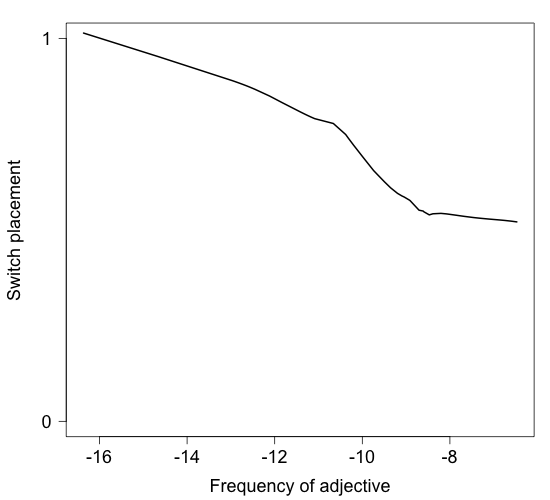
\includegraphics[scale=0.5]{figures/4-Fr_A_ru.png}
	\caption{The relationship between switch placement and frequency of the adjective. The values of 0 and 1 on the $y$-axis stand for switching within and outside the noun phrase, respectively. The frequency values on the $x$-axis are on the logarithmic scale.\label{fig:4:adj_ru}}
\end{figure}

The relationship between the languages of the examined adjective realisations and their frequency values is represented in Figure \ref{fig:4:adj_ru}. The horizontal axis is used for the frequency values of the adjectives under scrutiny, whereas the vertical axis is reserved for the dependent binary variable “switch placement”. Its values zero and one stand for a switch within the phrase and a switch at the phrase boundary, respectively. The switch is placed within the phrase when the adjective is realised in Russian, and it is located at the phrase boundary when the language of the adjective is German. The line depicting the relationship between the two variables is a Lowess curve, which represents a function describing the deterministic part of the variation in the data and is generated by locally weighted scatterplot smoothing, a local regression method \citep{lowess}. The near straight line, which is steadily inclined downward to the right, bends at two points: at $-10.68$ it begins to plunge sharply until its undulation point at $-8.48$, where it begins to plateau. This means that with the frequency of the adjective being low, the overall propensity is to select a German adjective and thus produce a German constituent. In other words, the likelihood for using a German adjective rises with the frequency of the adjective decreasing. The opposite also holds, namely, the higher the frequency of the adjective, the higher the probability of using a Russian adjective. However, at the log frequency of $-8.48$ or higher, no clear preference for the language of the adjective is observed.

Interestingly, several of the examined lexemes exhibit differing frequencies when determined in deWaC and when measured in the Russian corpus, which consists of the aforementioned Matusevich \textit{et al.} corpus and the RNC. Examples of such adjectives and their frequencies are given in Table \ref{tab:4:5}. We can infer from the table that some adjectives, such as \textit{normal} and \textit{normal'nyj}, \textit{klein} `small' and \textit{malen'kij} as well as \textit{letzt} `last' and \textit{poslednij}, occur in the German corpus at similar rates as in the Russian corpus, while others are used with differing frequencies. Among such adjectives we find  \textit{neu} `new' and \textit{novyj} as well as \textit{gut} `good' and \textit{xorošij}. The word \textit{neu} `new' appears 1.6 times more often in deWaC than its equivalent occurs in the Russian corpus, and the item \textit{xorošij} `good' is used 1.4 times more often in the Russian corpus than its equivalent in deWaC. Such recurrent lexemes, realised in Russian in one instance and in German in another instance, have quite different frequencies because their occurrences are counted in two different corpora. For example, the adjective \textit{nächst} in \textit{nächste Woche} `next week' has the frequency 12.92 on the logarithmic scale, whereas its Russian equivalent \textit{sledujuščij}, used in \textit{sledujuščaja Haltestelle} `next stop', has the frequency of 13.6. Based on these counts, when deciding between a German adjective and its Russian equivalent, the choice would be biased towards the Russian lexeme, only because its frequency was measured in another corpus. To avoid discrepancies between the utilised corpora, which may lead to inconsistencies in frequency counts, all frequencies are obtained from one and the same corpus. As German items form the bulk of the adjectives under scrutiny, it would be conclusive to use the German corpus as the only source of frequency values for the investigated items. For Russian items, translation equivalents are employed, so that the adjective `next', for example, has the frequency value 12.92 for each realisation: \textit{nächst} and \textit{sledujuščij}.

\begin{table}
		\begin{tabular}{lrr}
			\lsptoprule
			Lexeme realisations in Russian and German & \multicolumn{1}{c}{F\textsubscript{YM \& RNC}} & \multicolumn{1}{c}{F\textsubscript{deWaC}} \\\midrule
			`common' \textit{obščij} -- \textit{allgemein}	&3.901	&2.095\\
			`good' \textit{xorošij} -- \textit{gut}	&11.770	&8.164\\
			`last' \textit{poslednij} -- \textit{letzt} 	&6.526	&5.696\\
			`new' \textit{novyj} -- \textit{neu}		&9.282	&15.460\\
			`next' \textit{sledujuščij} -- \textit{nächst} 	&2.734	&4.257\\
			`normal' \textit{normal'nyj} -- \textit{normal}	&0.870	&0.862\\
			`small' \textit{malen'kij} -- \textit{klein}	&6.890	&5.940\\
			\lspbottomrule
		\end{tabular}
\caption{Russian and German realisations of the examined lexemes and their normalised relative frequencies in the German deWaC corpus and the Russian YM\&RNC corpora (i.e., the Matusevich et al. corpus and the Russian National Corpus).\label{tab:4:5}}
\end{table}

\begin{figure}
	\centering
    	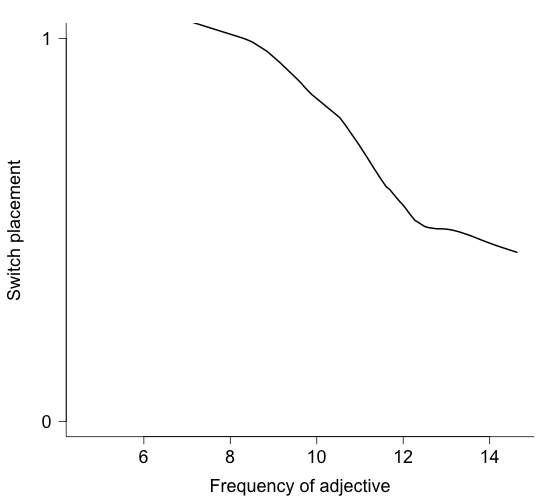
\includegraphics[scale=0.5]{figures/4-Fr_A_DEWAC.png}
	\caption{The relationship between switch placement and frequency of the adjective, as measured in deWaC. The values of 0 and 1 on the $y$-axis stand for switching within and outside the noun phrase, respectively. The frequency values on the $x$-axis are on the logarithmic scale.\label{fig:4:adj_de}}
\end{figure}

Figure \ref{fig:4:adj_de} illustrates the relationship between switch placement and the frequency of the adjective (see Appendix IV for the complete list of the examined items and the corresponding values). It is conspicuous that the shapes of the lines in Figures \ref{fig:4:adj_de} and \ref{fig:4:adj_ru} are analogous, although the slopes of the lines are different. This means that the frequency of the adjective exerts a similar effect on switch placement, regardless of the particular distribution in a given corpus. It therefore seems appropriate to use deWaC as a “benchmark” corpus. In doing so, I would be able to avoid possible inconsistencies in frequency counts owing to the differences in the given corpora and to thus ensure an adequate treatment of the adjectives by considering only the frequencies measured in the “benchmark” corpus.

To summarise, while low-frequency adjectives tend to be expressed in German, high-frequency adjectives exhibit a propensity to be realised in Russian, the matrix language. The analysis of frequency is conducted in the German and Russian corpora and shows that the frequencies with which the Russian and German realisations of several lexemes occur in the respective corpus may differ, depending on the utilised corpus. As argued above, in the subsequent statistical analysis I will consider only the frequencies obtained from the “benchmark” corpus, i.e., the German deWaC corpus, since the vast majority of the investigated adjectives are German.

\subsection{Frequency of the noun}
\begin{sloppypar}
Following the fact that frequent words are more accessible in language production and assuming that interactions between lexemes seem to control syntactic patterns \citep[][115]{macwhinney1997}, we could hypothesise that frequent words can activate lexico-grammatical patterns in which they occur faster than rare words. In other words, lexico-grammatical patterns associated with frequent words, such as collocations and more abstract syntactic constructions, may be highly accessible. In the context of this chapter, high-frequency German nouns are assumed to trigger their typical adjective collocates more often than low-frequency nouns. Hypothesis testing again involves corpus analysis. Since all the nouns involved in the noun phrases under investigation are German, their frequencies were determined in the deWaC corpus. Table \ref{tab:4:6} illustrates examined noun phrases whose nouns occur with the highest and lowest frequencies in deWaC. As shown in the table, both frequent and rare German nouns may combine with German adjectives on a regular basis. We can thus conclude from the few instances given that identifying a tendency in each of the groups seems to be impossible. However, a large-scale comparison may be promising.
\end{sloppypar}

\begin{table}
		\fittable{\begin{tabular}{lr} 
			\lsptoprule
			Noun phrases	& \multicolumn{1}{c}{F\textsubscript{N}} \\\midrule
			konkretnyj \textit{Meister[lehr]gang} `concrete master craftsman's course'	&33\\
			\textit{gefundene Kneipentour} `invented pub-crawl'		&147\\
			\textit{ausgebildeter Polizeihund}	`trained police dog'	&180\\
			\textit{Weinblätter gefüllt} `filled vine-leaves'	&266\\
			krasivyj \textit{Saunalandschaft} `beautiful sauna facilities'	&313 \\
			\midrule
			normal'naja \textit{Arbeit} `normal work'		&635,026\\
			\textit{letzte Arbeit} `last work'	&635,026\\
			\textit{soziales Jahr} `gap year for social work'	&1,034,532\\
			\textit{freiwilleges Jahr} `volunteer gap year'	&1,034,532\\
			\textit{nächstes Jahr} `next year'	&1,034,532\\
			\lspbottomrule 
		\end{tabular}}
\caption{German and mixed noun phrases, ranked in order of lowest (above) and highest (below) frequencies of the nouns involved.} \label{tab:4:6}
\end{table}

\begin{sloppypar}
An examination of the relation between the frequency of the noun and switch placement is represented in Figure \ref{fig:4:noun}. The logarithmically transformed frequency of the noun is on the horizontal axis, whereas the vertical axis is reserved for the dependent binary variable “switch placement”, as is the case with the previously discussed factor. The values zero and one of the dependent variable stand for a switch within the phrase and a switch at the phrase boundary, respectively. The curve representing the relationship between the two variables is a Lowess curve (see \ref{section_fr_adj}). Although the line has several inflection points, most of it runs roughly parallel to the \textit{x}-axis. The line begins to curve upwards only at the point of 10.2 on the log scale (i.e., the frequency of 26,903 in deWaC). In other words, noun frequency seems to influence switch placement only in the range of frequent words, which exhibit the frequency of 26,903 or higher in the given corpus. This means that recurrent nouns co-activate lexemes that regularly combine with them in German. As a result, the noun phrase is realised in German and the switch is placed at the phrase boundary. However, a reverse effect for low-frequency nouns cannot be found. In order to establish the relevance of the factor “noun frequency” for contributing to the overall variance in the data, a  multifactorial analysis is conducted below.
\end{sloppypar}

\begin{figure}
    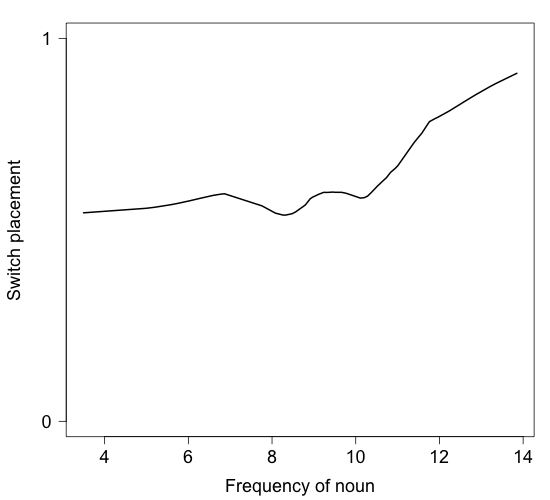
\includegraphics[scale=0.5]{figures/4-Fr_N.png}
	\caption{The relationship between switch placement and frequency of the noun. The values of 0 and 1 on the $y$-axis stand for switching within and outside the noun phrase, respectively. The frequency values on the $x$-axis are on the logarithmic scale.\label{fig:4:noun}}
\end{figure}

In summary, lexical frequency does appear to play a role in code-mixing. German adjective-noun combinations seem to be inserted into Russian sentences when their adjectives exhibit low frequencies and their nouns are on the contrary high-frequency words. However, the frequencies with which the parts of such a combination appear in a German corpus may be insufficient for explaining multiword insertions. The crucial factor responsible for the occurrence of multiword insertions in code-mixing could rather be their unit status in the corresponding language. 

In order for a word combination to count as a multiword unit, or a chunk, the words comprising it have to appear together with a relatively high frequency. Such recurrent word combinations exhibit not only syntagmatic stability but also semantic coherence \citep[cf.][136]{bybee-book-2010}. In a defined linguistic context, such as the adjective-modified noun phrase, corpus frequency of a word combination, or word string frequency, may be a reliable indicator of its unit status \citep[][]{heylen-2014}. Nevertheless, word string frequency is a controversial metric for determining multiword units. For example, based on psycholinguistic judgements of unithood, \citet{simpson.vlach&ellis2010} assert that Mutual Information (MI), a statistical measure of association, provides a better grip on semantically coherent units than word string frequency. In an attempt to underpin the nature of multiword insertions in code-mixing, subsequent analysis will consider both measures of semantic coherence:  frequency of co-occurrence and mutual information.  

\subsection{Frequency of co-occurrence}
Following Bybee's (\citeyear[112]{bybee-constituency-2002}) Linear Fusion hypothesis, which states that ``items used together fuse together'', switch placement in the context of the adjective-modified noun phrase can be assumed to be a function of the frequency with which specific adjectives and nouns appear together in the corresponding language. \citet{diessel-toappear} attributes this effect to automatisation, which can be defined as a cognitive mechanism whereby sequential activities become uncontrolled, automatic processes\footnote{\citet{bybee-book-2010} uses the term \textit{chunking} instead of \textit{automatisation}}. According to \citet{diessel-toappear}, linguistic elements, which naturally occur in sequence, represent sequential information and are thus subject to automatisation. Repetition of strings of linguistic elements leads to the gradual emergence of processing units, or chunks of linguistic elements.  The view of chunks as units emerging from usage processes needs to be complemented by the consideration that many chunks are rote learnt as units already in the process of language acquisition (see Chapter \ref{UBL}, for details). In this vein, it could be argued that in the context of the adjective-modified noun phrase, a particular adjective and a specific noun exhibit a strong sequential link and form a unit if the frequency with which this noun is used with the adjective is high. I hypothesise that in code-mixing, a switch in such a unit would be unlikely (cf. \citealt[125--131]{backus-two-1996} and \citealt[386]{boumans-syntax-1998}, who come up with similar suggestions but do not subject them to systematic analysis). Conversely, if the association between an adjective and a noun is weak, i.e., they appear together at a low rate, the probability of a switch between them is high.\footnote{These hypotheses may be related to the work investigating disfluency placement in spontaneous speech \citep[e.g.,][]{schneider2014}.} Testing these hypotheses required obtaining co-occurrence frequencies of the examined adjective-noun combinations in deWaC. 

The corpus analysis of German adjective-noun combinations was straightforward. The frequency of a specific adjective-noun combination was determined by counting its occurrences in deWaC, while disregarding some of the variability in its morphological forms on purpose. This variability pertains, in the first place, to the modifying adjective, since its form depends not only on the morphological case marked on the noun phrase but also on the presence/absence of preceding determiners. For example, the phrases \textit{nächst-es Jahr} `next year', \textit{(das) nächst-e Jahr}, \textit{(dem) nächst-en Jahr} involve the same lexical items \textit{nächst} and \textit{Jahr} but exhibit differences in the marking of the adjective.\footnote{The only morphological contrast between singular noun forms is the distinction between the genitive case and the non-genitive cases. The only difference between plural noun forms is the opposition between dative and non-dative forms. Yet, case marking on the noun was also discarded.} Nevertheless, they are all considered instantiations of one specific underlying collocation for two reasons. First, the combination of these words is syntagmatically stable, \textit{i.e.,} $[$ {(\textsc{det}) \textit{nächst}-\textsc{agr}} \textit{Jahr}(-\textsc{gen}) $]$, and second, its overall frequency in the corpus is high. As concerns the grammatical number, items differing in this category were handled separately.\footnote{Corpus linguistic studies provide tangible evidence that different number values of a noun may frequently result in different collocation sets \citep[e.g.,][167--172]{sinclair2003}. That is, singulars and plurals may display different collocational tendencies.} On this account, only the morphological variants of the underlying collocation in the singular, or in the plural were taken into consideration; their individual frequencies were added together. The same procedure applied to mixed noun phrases, headed by German nouns and modified by Russian adjectives, the only difference being in the use of German equivalents of the Russian adjectives.

The results for ten most frequent adjective-noun combinations are reported in Table \ref{tab:4:7}. As is seen from the table, high-frequency adjective-noun combinations mostly but not invariably repel switching. The combination \textit{sledujuščij Tag} `next day' is the only adjective-noun combination in the table that is not produced as a holistic unit but is interrupted by a switch. However, the general tendency is in favour of the proposed hypothesis. The converse hypothesis that code-switches tend to occur in noun phrases between adjectives and nouns if these adjective-noun combinations are infrequent also seems to hold, although not all the data support it. Recall that according to this hypothesis, German low-frequency combinations will not emerge in bilingual sentences, and only mixed combinations, with more accessible Russian adjectives, will be produced instead. Adjective-noun combinations whose co-occurrence frequencies, as determined in deWaC, are in the lowest range are listed in Table \ref{tab:4:8}. (It is important not to forget that for combinations of German nouns with Russian adjectives, German equivalents of the actual adjective realisations were used.) The table contains five adjective-noun combinations in which both words are realised in German and five combinations in which only the nouns are German. Judging by the low frequencies of these combinations, it could be argued that they represent free word combinations. Such combinations are essentially unconstrained lexically, and therefore, the adjectives in them may be expressed either in Russian, or in German. An exception to this tendency is the combination \textit{ausgebildeter Polizeihund} `trained police dog', which may be regarded as a lexical chunk by virtue of its high semantic coherence, and we can possibly get a grip at this chunk when another measure, such as Mutual Information, is utilised to model the strength of association between words. This will be done in the next section.

\begin{table}
		\begin{tabular}{lr}
		    \lsptoprule
			Noun phrases	& \multicolumn{1}{c}{F\textsubscript{A-N}} \\ \midrule
			\textit{nächstes Jahr} `next year'	&27785\\
			sledujuščij \textit{Tag} `next day'	&22927\\
			\textit{katholische Kirche} `Catholic Church'	&20856\\
			\textit{nächste Woche}	`next week'	&10499\\
			\textit{erstes Semester} `first term'	&3185\\
			\textit{gute Nacht} `good night'	&3031\\
			\textit{nationale Idenitität} `national identity'	&2878\\
			\textit{alte Bundesländer} `old federal states (of Germany)'	&1445\\
			\textit{letzte Arbeit} `last work'	&1262\\
			\textit{bares Geld} `cash money'	&1148\\
			\lspbottomrule 
		\end{tabular}
\caption{German and mixed noun phrases, ranked in order of their frequencies in the deWaC corpus.\label{tab:4:7}} 
\end{table}

\begin{table}
		\begin{tabular}{lr}
		\lsptoprule
			Noun phrases	& \multicolumn{1}{c}{F\textsubscript{A-N}} \\\midrule
			\textit{russische Party} `Russian party'		&3\\
			krasivyj \textit{Saunalandschaft} `beautiful sauna facilities'	&3\\
			\textit{ausgebildeter Polizeihund} `trained police dog'	&3\\
			bednyj \textit{Hausmeister} `poor caretaker'		&2\\
			real'naja \textit{Schlampe} `real slut'	&2\\
			\textit{Schlampe} redkostnaja `rare slut'		&2\\
			\textit{normales Klo} `normal loo'	&1\\
			\textit{lebendes Fragezeichen} `living question mark'	&1\\
			novyj \textit{Trockner} `new drier'	&1\\
			\textit{süße Grußkarte} `sweet greeting card'	&1\\
			\lspbottomrule
		\end{tabular}
\caption{German and mixed noun phrases, ranked in order of their frequencies in the deWaC corpus.\label{tab:4:8}} 
\end{table}

The corpus analysis revealed that some of the German noun phrases with adjective modifiers do not occur in deWaC. Among them are the following phrases: \textit{chillige Familie} `relaxed family', \textit{freie Bundesländer} `free federal states' (in reference to the highly autonomous estates of the Holy Roman Empire) and \textit{gefundene Kneipentour} `found pub crawl' (\textit{gefunden} `found' is possibly confused with \textit{erfunden} `devised'). Furthermore, German equivalents of the following mixed phrases are not attested in the corpus: \textit{ogromnyj Titel} `huge header' (G \textit{riesig}), \textit{sportivnye Sachen} `sporty things' (G \textit{sportlich}), \textit{russkij Besitzer} `Russian owner' (G \textit{russisch}), \textit{obščij Hochdeutsch} `general Standard German' (G \textit{allgemein}) and \textit{konkretnyj Meistergang} (the word \textit{Meistergang} is not found in the corpus itself, but the conversation context clarifies the use of this word: the speaker substitutes the word \textit{Meisterlehrgang} with the given shorter form) `concrete master craftsman's course' (G \textit{konkret})\footnote{It is noteworthy that neither was the collocation \textit{konkreter Meisterlehrgang} attested in the corpus.}.

\begin{figure}
    	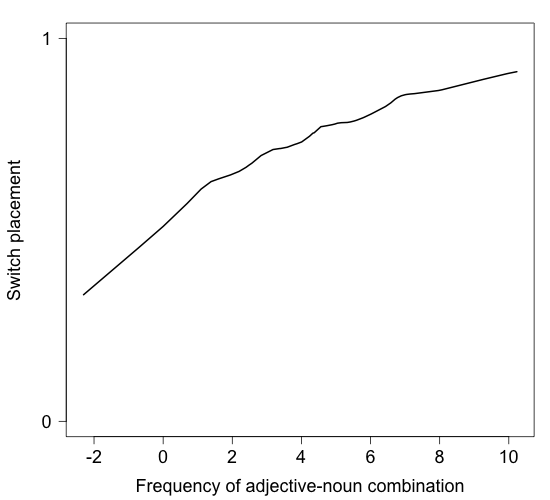
\includegraphics[scale=0.5]{figures/4-Fr_co-occ.png}
	\caption{The relationship between switch placement and frequency of adjective-noun combinations in deWaC. The values of 0 and 1 on the $y$-axis stand for switching within and outside the noun phrase, respectively. The frequency values on the $x$-axis are on the logarithmic scale.\label{fig:4:co-occ}}
\end{figure}

The relation between switch placement and the frequency of an adjective-noun combination, or co-occurrence frequency, is plotted in Figure \ref{fig:4:co-occ}. The horizontal axis is reserved for the frequency of co-occurrence, whose values are logarithmically transformed, whereas the vertical axis is used for the binary variable “switch placement”. As in the previous figures representing the relationships between switch placement and frequency distributions (see, for example, Figure \ref{fig:4:adj_de}), the line depicting the relationship between the two variables is a Lowess curve. The curve, which is inclined upwards to the right, demonstrates that with growing co-occurrence frequency, an across-the-board gradual increase in probability for placing a switch at the phrase boundary is expected. The absence of dramatic inflection points on the curve signifies that the tendency is stable over the whole line. In other words, the higher the frequency with which a specific noun is used with an adjective, the more likely a switch at the boundary of the extended noun phrase. This finding may be viewed as a confirmation of the Linear Fusion hypothesis; that is, if two words appear together with a high frequency, they form a multiword unit, which is activated as a whole in production. Additionally, by using the complete data for the correlation between switch placement and frequency of co-occurrence, evidence could be found in support of the reverse hypothesis, according to which a switch between an adjective and a noun is likely if the association links between them, as determined by co-occurrence frequency, are loose, or non-existent. It should be noted however that certain strings which may well count as lexical chunks, as reported above, could not be detected by the application of co-occurrence frequency as a measure of associations between words. Another method of measuring association strength, namely, Mutual Information, will be employed below, in order to get a better grip at all types of lexical chunks.

\subsection{Mutual Information}

As reported in studies on lexical production and comprehension, ``mutual information is a better measure of the cohesion for two-word pairs'' \citep{gregory-etal-1999} than co-occurrence frequency \citep[cf.][]{ellis-formulaic-2008}. Mutual information is a statistic measure drawn from information science aimed at assessing the extent to which the words in a pair appear together more frequently than would be expected by chance \citep{oakes-1998, manning-schuetze-1999, wiechmann-2008}. According to \citet{fano-1961}, if two words, $x$ and $y$, have probabilities $P(x)$ and $P(y)$, then their mutual information (MI), $I(x,y)$ is defined to be \[ I(x, y) = \log_2 \frac{P(x,y)}{P(x)P(y)} \]

\noindent An informal definition is this: ``mutual information compares the probability of observing $x$ and $y$ \textit{together} (the joint probability) with the probability of observing $x$ and $y$ \textit{independently} (chance)'' \citep[23]{church-hanks-1990}. A higher MI score stands for a stronger cohesion between the words, while a lower score means that their co-occurrence is rather due to chance. The formula was modified as suggested in \citet{wiechmann-2008}: \[  \text{MI} = \log_2 \frac{P(x,y)}{P(x)P(y)}N \]  where \textit{N} signifies the number of words in the corpus. This modification does not alter the relations in the formula, but raises the scores and thus allows a more straightforward comparison. In terms of the investigated data, $P(x)$ and $P(y)$ stand for the frequency of the adjective and the frequency of the noun, respectively, and $P(x,y)$ represents the frequency with which the adjective and the noun co-occur.\footnote{With the intention of not omitting unattested adjective-noun combinations from the data set, the frequency of a combination which is not attested in deWaC was set as 0.1, rather than 0. This allowed a differentiation between unattested and very rare combinations in deWaC.}

Table \ref{tab:4:9} contains inserted German noun phrases distinguished by the highest MI scores in the data set. The words in each of the pairs from the table are strongly associated with each other: each word pair expresses a very specific meaning. The meaning of one word combination, i.e., \textit{fauler Sack} `lazy git', is even idiomatic. However, as evident in the table, the other word pairs exhibit compositional but still very specific meanings. Consequently, a close semantic relation between the words in a word pair appears to support the sequential link between them. In other words, the examined noun and adjective lexemes cohere on semantic grounds into multiword units. Observing the word pairs in the table, we can assert that in bilingual speech, both words in each pair are indeed realised in the same language, i.e., German.

\begin{table}
		\begin{tabular}{lr}
		\lsptoprule
			Noun phrases	& \multicolumn{1}{c}{MI} \\\midrule
			\textit{Weinblätter gefüllt	} `filled vine-leaves'	&15.32\\
			\textit{standesamtliche Hochzeit} `civil wedding ceremony'	&11.22\\
			\textit{gebratene Nudeln} `fried noodles'	&11.01\\
			\textit{gefüllte Paprika} `filled pepper'	&10.50\\
			\textit{alleinerziehende Mutter} `single mother'	&10.42\\
			\textit{ausgebildeter Polizeihund}	`trained police dog'	&10.32\\
			\textit{katholische Kirche} `Catholic Church'	&10.30\\
			\textit{fauler Sack} `lazy git'		&10.23\\
			\textit{gehackte Tomaten} `chopped tomatoes'	&10.16\\
			\textit{bares Geld}	 `cash money'	&10.14\\
			\lspbottomrule 
		\end{tabular}
\caption{Inserted German noun phrases with highest MI scores in data set.\label{tab:4:9}} 
\end{table}


Table \ref{tab:4:10} lists the noun phrases which exhibit the lowest MI scores in the data set. Most of the given noun phrases are mixed constituents, though three of them are German insertions. We may thus conclude that mutual information appears to account for switch placement in a large part of the data, but not in every instance. While highly coherent phrases with high MI scores repel internal switches, phrases with low MI scores in German apparently tend to attract them. Since this effect is gradual and best conceived as a tendency, it will be tested statistically in the remainder of this chapter.

\begin{table}
		\begin{tabular}{lr}
		    \lsptoprule
			Noun phrases	& \multicolumn{1}{c}{MI} \\ \midrule
			\textit{erster Freund}	`first (boy)friend' &0.6626524\\
			novyj \textit{Trockner} `new drier'		&−0.7394403\\
			klassnoe \textit{Sprache} `cool language' 	&−0.7835933\\
			\textit{gute Geschäftsführung} `good management'	&−1.0246024\\
			obščij \textit{Hochdeutsch}	 `general Standard German'	&−1.2734782\\
			russkie \textit{Begriffe} `Russian terms'	&−1.3562067\\
			sportivnye \textit{Sachen} `sporty things'	&−4.7012769\\
			\textit{freie Bundesländer} `free federal states' &−6.8530364\\
			ogromnyj \textit{Titel}	 `huge header'	&−7.0364000\\
			russkij \textit{Besitzer} `Russian owner'	&−7.6235176\\
			\lspbottomrule 
		\end{tabular}
\caption{Inserted and mixed noun phrases with lowest MI scores in data set.\label{tab:4:10}}
\end{table}

As regards the lexical items involved in the noun phrases with very low mutual information, we can observe that one of the words in a pair is often a high-frequency word. It may either be the adjective, such as \textit{novyj} `new' in in the combination \textit{novyj Trockner} `new drier' and \textit{gut} `good' in \textit{gute Geschäftsführung} `good management', or the noun, such as \textit{Begriffe} `terms' in \textit{russische Begriffe} `Russian terms' and \textit{Sachen} `things' in \textit{sportivnye Sachen} `sporty things'. Since the frequency of these lexemes is high, a chance that they combine with other words is also high. As a result, these strings exhibit low degrees of cohesion and therefore low MI scores. Of particular relevance in the discussion of mutual information is Oakes' (\citeyear{oakes-1998}) cautionary assertion that ''[t]his measure gives too much weight to rare events'' (p. 171). The MI scores of some rare and unusual word co-occurrences can indeed be higher than the scores of certain frequent and semantically more coherent word combinations. Hence, the adjective-noun combinations \textit{süße Grußkarte} `sweet greeting card' and \textit{schöne Saunalandschaft} `beautiful sauna facilities' (whose adjective is realised in Russian in the bilingual corpus) have the scores of 7.142 and 4.788, whereas such word combinations as \textit{gute Ablenkung} `good diversion' and \textit{(freiwilliges) soziales Jahr} `(voluntary) gap year for social work' have considerably lower MI scores, i.e., 3.239 and 0.969, respectively. For this reason, it is crucial to investigate the correlation between mutual information and the speakers' preferences in switch placement on a large scale.

\begin{figure}
    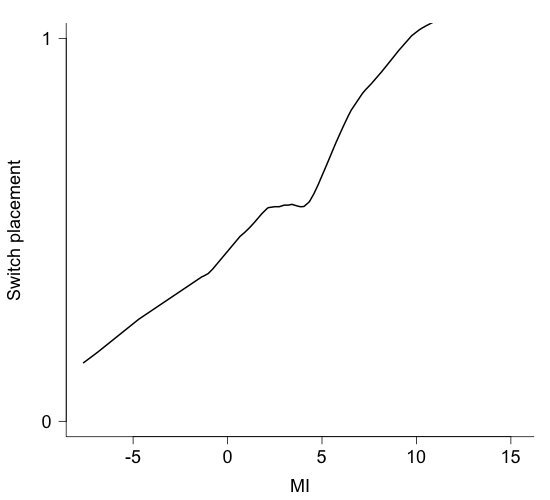
\includegraphics[scale=0.5]{figures/4-MI_de.png}
	\caption{The relationship between switch placement and the mutual information (MI) of adjective-noun combinations in deWaC. The values of 0 and 1 on the $y$-axis stand for switching within and outside the noun phrase, respectively.}
	\label{fig:4:MI_de}
\end{figure}

Figure \ref{fig:4:MI_de} plots the correlation between MI and switch placement. In the graph, MI scores of the investigated co-occurrences are on the horizontal axis and switch placement is on the vertical axis. The line representing the relation between the two variables is a Lowess curve (cf. Figure \ref{fig:4:adj_ru}). As is visible in the graph, the line displays a steep and steady upward trend for placing the switch at the phrase boundary, except for the interval between the scores of 2.14 and 4.0, where this trend levels off. In this interval, the switch may be placed either within or outside the noun phrase with a fifty-fifty chance. On the whole, however, the graph reveals a strong tendency for switching at the phrase boundary, with mutual information increasing, which appears to support the aforementioned research hypothesis. Yet, the question whether the factor MI is particularly pertinent to explaining the overall variance in the data is open to statistical investigation. Thus, the remainder of this chapter is occupied with the statistical modelling of the investigated factors and their interplay.

\section{Statistical prediction of switch placement}\label{4:stat}

As the examined factors compete and interact with each other online in determining switch placement in noun phrases with adjective modifiers, it is crucial to account for their individual contributions as well as their interplays by using logistic regression analysis, which calculates the effect of individual predictors on a binary dependent variable under multivariate control. In terms of the investigated patterns of switch placement, this statistical method allows to determine the probability with which a switch is placed within the modified noun phrase or at its boundary given the conditioning factors discussed in the previous section as well as the importance of each of these factors. The generalised linear mixed-effects model, which I use in the present and the subsequent chapters, does this through the investigation of both fixed and random effects (see \citealt[278--84]{baayen-analyzing}; cf. \citealt{bresnan-etal}).

A fixed-effect factor exhausts all of its possible levels, each of which can in principle be repeated. The fixed-effect factors in my data are measured numeric factors, such as frequency and mutual information. Random-effect factors have the property that they usually represent a random selection of the levels available in the population from a potentially infinite number of levels, or instances \citep[][241]{baayen-analyzing}. The individual levels of these factors are not interesting per se in a statistical analysis. The random-effect factor in my analysis is Individual. Since individual speakers contribute varying numbers of observations to the data set, the speaker may become a very influential factor \citep[][]{tagliamonte-baayen-2012}, capable of distorting the effect of the fixed-effect predictors, and has therefore to be treated as a random-effect factor. According to \citet[158]{tagliamonte-baayen-2012}, ``[a]n important advantage of the mixed-effects modeling framework is that it allows the researcher to sample as many tokens from a given individual as is feasible, thereby increasing statistical power''. 

The statistics package R version 2.12.0 \citep{r} was used to carry out logistic regression analysis and all other statistical tests, and to generate graphical plots.

In a regression model with mixed effects, the joint contribution of all factors is computed by testing each factor individually, while the other factors remain constant. There are various search procedures for determining the model that provides the best fit to the data \citep[cf.][]{baayen-2013}. In selecting one of the customary heuristics, I adopt forward stepwise model selection. The general procedure of this method consists in successive adding of potentially relevant predictors to the model specification. Applied to the factors outlined in the previous section, frequency of the adjective was the first fixed-effect factor included in the regression model, then the other factors, which include various frequency measures, were added stepwise. The models were compared in terms of Akaike's information criterion (AIC), which estimates a model's accuracy and complexity. Decreases in values of AIC indicate a better fit of the model. The minimal adequate model is rather accurate: as detailed in Table \ref{tab:4:11}, it correctly classifies 82 per cent of all instances of switch placement in the data set, while the baseline model, which always predicts the most frequent realisation, i.e., switch placement at the phrase boundary, is only accurate in 65 per cent of cases. This shows the model's considerable increase in accuracy over the baseline model. The model delivers 86.7 per cent of correct predictions of switches placed at the phrase boundary; the prediction of switch placement within the noun phrase is more difficult since the model predicts this variant correctly in 74.2 per cent of cases. The  model is reported in Table \ref{tab:4:12}. The \textit{C} index, estimating the probability of concordance between predicted and observed choices, is 0.903, which signals a high predictive power of the model. The performance indicator Somer's Dxy amounts to the value of 0.805, indicating a good fit. The model predictors exhibit a negligible degree of collinearity: the condition number κ, used for assessing collinearity, is 12.1 and thus below the threshold indicating medium collinearity \citep[cf.][182]{baayen-analyzing}. This is especially encouraging in view of the fact that the model's both predictors are frequency measures, which generally tend to be highly collinear \citep{baayen-2013}.

\begin{table}
		\begin{tabular}{l *{4}{r}} 
		\lsptoprule
 			& & \multicolumn{2}{c}{Predicted} & \% correct\\\cmidrule(lr){3-4}
			  & &0 &1 &\\ \midrule
			Observed  & 0     &23   &8 &74.2\\
			 &1 &8 &52 &86.7\\
			 & & &Overall &82.0\\
			 \lspbottomrule
		\end{tabular}
\caption{Model accuracy. Classification table for the model (1: switch at the phrase boundary; cut value = 0.50). (The table representation is based on   \citealt{bresnan-etal}.)\label{tab:4:11}}
\end{table}

\begin{table}
\begin{tabular}{l rrrr l}
		 \lsptoprule
            	Factor & \multicolumn{1}{c}{Est.} & \multicolumn{1}{c}{SE} & \multicolumn{1}{c}{$z$}  & \multicolumn{1}{c}{$\text{Pr}(>|z|)$} & \\\midrule
			(Intercept)  &10.237 &2.795 &3.662 &$<0.001$ &{***}\\
			Frequency of A &−0.919 &0.233 &−3.954  &$<0.001$ &{***}\\ 
			Co-occurrence fr. &0.374 &0.109   &3.422 &0.001 &{***}\\\midrule
			\multicolumn{6}{l}{Random effect:}\\
			\multicolumn{6}{l}{Speaker}\\
			\multicolumn{6}{l}{(intercept, $N = 17, \text{variance} = 0.999, \sigma = 0.999$)}\\
			\midrule 
			\multicolumn{6}{l}{Summary statistics:}\\
			\multicolumn{2}{l}{$N$} & 91\\
			\multicolumn{2}{l}{\% correct predictions (\% baseline)}  & 82 (65)\\
			\multicolumn{2}{l}{\textit{C} index of concordance}  & 82 (65)\\
			\multicolumn{2}{l}{Somer's Dxy}  & 0.805\\
			\lspbottomrule
		\end{tabular}
\caption{Predicting switch placement in the context of the noun phrase modified by an adjective: minimal adequate generalised liner mixed model. Predicted odds are for switch placement outside the noun phrase. Significance codes: *significant at $p<0.05$, ** $p<0.01$, *** $p < 0.001.$ \label{tab:4:12}}
\end{table}

Let us now inspect the predictors in the reported model. The predicted odds are for switch placement outside the modified noun phrase:  positive coefficients indicate that a factor favours placing switches at the constituent's boundary, negative coefficients indicate that a factor attracts switch placement within the modified noun phrase, i.e., between the adjective modifier and the head noun. Hence, the frequency with which an adjective and a noun co-occur enhances the probability for a switch at the phrase boundary, whereas the frequency of the adjective reduces this probability. The coefficients are on the log scale and may be used to calculate the probability of switch placement outside the phrase in every case, as suggested in \citet{ehret-etal-2014}. The line `Intercept' provides the log odds in the default case, which occurs when the frequency of an adjective-noun co-occurrence is average and the adjective has a low average frequency. An example from the bilingual corpus that comes closest to the default case is \textit{türkise Farbe} `turquoise colour', both its frequency and the frequency of its adjective are quite low in deWaC. For the default case, the model yields log odds of 10.24. We can interpret this value as odds if we reverse the natural logarithm \citep[cf.][]{ehret-etal-2014}. Hence, the odds are 27887.63 and the associated probability of placing the switch outside the noun phrase is 0.999. The odds for the estimated coefficients of the predictor variables are calculated in the same fashion. Thus, for co-occurrence frequency the odds ratio is 1.455, which means that while holding the other predictor constant, the likelihood for inserting a German noun accompanied by a German adjective in an otherwise Russian sentence grows by approximately 50 per cent at every one-unit increase of co-occurrence frequency on the logarithmic scale. This corresponds an increase by around 7 correctly predicted tokens on the linear scale. In other words, if the frequency with which a noun and an adjective appear together in German grows by 7 tokens, the odds for inserting an adjective-noun combination enhance by 50 per cent. 

Frequency of the adjective has a lesser effect size than co-occurrence frequency. Although being a less strong predictor, frequency of the adjective is nevertheless the most important predictor of the observed variation. A model including the factor frequency of the adjective as the only fixed-effect factor has the lowest AIC in comparison to similar models testing one of the four investigated factors -- MI, frequency of the adjective, frequency of the noun and co-occurrence frequency -- as a single predictor. For the factor frequency of the adjective, odds were determined to be 0.39 on the linear scale. This means that increasing the frequency of the adjective by one unit lowers the expected percentage of switches placed outside the noun phrase by around 40 per cent. If the adjective is a high frequency word and the frequency of co-occurrence is particularly low, the chance for switching the language within the noun phrase is high, as in the case of \textit{ogromnyj Trockner} `huge drier' and \textit{russkij Besitzer} `Russian owner'. Conversely, if an adjective is infrequent and the frequency with which an adjective and a noun co-occur is high, the trend is towards inserting this adjective-noun co-occurrence into an otherwise Russian sentence, as in the case of \textit{bares Geld} `cash money' and \textit{alleinerziehende Mutter} `single mother'.

With regard to the random-effect predictor speaker, we can assert judging by its variance and the corresponding standard deviation that differences among the speakers in the corpus in terms of their preference for one of the two switching patterns are negligible. The highest adjustment to the model's intercept (1.34) is observed with the speaker who contributes most instances of switching in the context of the modified noun phrase to the data set. She exhibits a marked preference for placing switches at the phrase boundary.

In sum, the statistical regression analysis enabled discrimination between the examined usage-based factors in terms of their contribution to explaining the variation in switch placement in the data. Of the four analysed predictors -- frequency of the adjective, frequency of the noun and frequency of the adjective-noun co-occurrence and mutual information -- frequency of the adjective and co-occurrence frequency were found to account for switch placement in the context of the adjective-modified noun phrase. Although mutual information appeared to have a high predictive power, when included as the only fixed-effect predictor in the model's term, frequency of the adjective performed better in the respective model under the same conditions. Adding MI to the final, minimal adequate regression model, which was based on co-occurrence frequency and frequency of the adjective, did not result in an improvement of the model quality. The variation under scrutiny can thus be captured by usage-based factors such as the frequency of the adjective, as measured in a German corpus, the frequency with which the noun and the adjective appear together in the same corpus, and the factor speaker, handled as a random effect predictor.

\section{Conclusions and discussion}

Already the early systematic studies of bilingual speech, such as \citet{pfaff-constraints-1979} and \citet{poplack-sometimes-1980} report insertion of nominal constituents from one language in contact into the other and emergence of their code-mixed counterparts. As outlined above, the nature and status of inserted nominal constituents are a matter of controversy. Although some previous work (\citealt{backus-two-1996, boumans-syntax-1998}) has acknowledged the importance of recurrent combinations of words for the structure of code-mixing, no systematic evidence has been gathered to date to substantiate or refute this claim. Thus, the aim of this chapter has been to examine these two kinds of nominal constituents in detail to show that the choice between them depends on lexical factors, such as collocational ties between words and word frequency, rather than structural non-equivalence, as previously assumed \citep{myers-scotton-matching-1995,myers-scotton-contact-2002}.

The analysis of Russian-German code-mixing showed that German adjective-noun combinations are frequently inserted in Russian sentences. A vast majority of them represent well-formed German nominal constituents, of which only a fraction are fully-fledged German noun phrases. Crucially, a great number of adjective-noun combinations are inserted in Russian sentences without German determiners, but their internal structure is yet analysable since gender-number agreement is largely maintained. The tendency to omit determiners while preserving the internal structure of the nominal constituents is interpreted as a strategy to enhance structural similarity between the languages involved in code-mixing (cf. \citealt[][]{hakimov-backus-20-intro};  \citealt[][]{sebba-09}). However, not all of the inserted adjective-noun combinations represent well-formed German nominal constituents. Since words in these constituents may be subsequent insertions, rather than parts of a multimorphemic insertion, only well-formed German constituents from bilingual sentences were subject to subsequent analysis. 

Another bilingual strategy to express an adjective-modified noun phrase is to produce a mixed constituent. In my bilingual corpus, German noun insertions regularly combine with Russian attributive adjectives, but modification of Russian nouns by German attributive adjectives was not attested. Adjective-modified nominal constituents in the analysed bilingual speech have thus German nouns as heads, and both German and Russian attributive adjectives as modifiers. In other words, a bilingual speaker may switch from Russian to German either inside the adjective-modified nominal constituent, or at the constituent boundary,  producing an embedded-language island.

The choice between these two patterns of switch placement was hypothesised to depend on the following factors: frequency of the adjective, frequency of the noun, frequency of their co-occurrence and mutual information, a statistical measure of association between them. The speakers' possible predilections towards one of the patterns was controlled for using the random factor “individual” in the analysis. Corpus linguistic methodology and statistical modelling were used to test the contribution of each of the factors to explaining the variation in the data set.

The findings of the study include two frequency effects. Occurrence frequency of adjectives appears to affect switch placement in the adjective-modified noun phrase in my data. Frequent, more accessible adjectives tend to come from Russian, which is the language of the sentence frame and is thus the more activated language in this case. Attributive adjectives of average or low frequency, which exhibit very specific meanings, are predominantly German. This observation provides evidence for \citeauthor{backus-evidence-1999}’s (\citeyear{backus-evidence-1999},\citeyear{backus-units-2003}) specificity continuum hypothesis introduced in \sectref{section_fr_adj}, according to which in bilingual speech, items from another language usually have specific meanings, particularly at early stages of contact, as is the case in the current study. As regards online production, we may conclude that whenever a very specific German adjective of average or low frequency is activated and accessed, it co-activates, or triggers, the head noun in the same language. This may be to the fact that in German, an inflected adjective sets a strong projection with regard to the nature of the following element, which must be a noun (\citealt[][98]{auer_syntax_2007}; \citealt[cf.][]{auer_projection_2005}). It is important to emphasize that co-activation spreads from the adjective to the noun and not vice versa because not a single German adjective appears to modify a Russian noun in these data, i.e., each inflected German adjective is followed by a German noun, but German nouns freely combine with Russian adjectives. These results shed light on the degrees of activation of the German lexicon/grammar during the processing of the examined constructions. As the adjectives modifying German nouns in otherwise Russian sentences are mainly German and their accessibility in processing, owing to their low and average frequencies of use, is restricted, we may assume that the German lexicon/grammar is highly activated when German nominal constituents, or the so-called Embedded-Language islands, are produced. In other words, the German lexicon/grammar should be more strongly activated because it delivers very specific adjectives and is also responsible for the co-activation effect. When the role of German is restricted to supplying only nouns involved in mixed nominal constituents, its activation seems to be lower. Hence, the effect of the lexical frequency on the choice between a German monolingual constituent and a mixed Russian-German constituent offers indirect support for \citeauthor{myers-scotton-contact-2002}’s (\citeyear[][140]{myers-scotton-contact-2002}) view that the production of embedded-language islands and the production of single embedded-language elements occurring in the matrix language frame require different levels of activation of the embedded language.

That frequency with which nouns and adjectives are used together in German influences switch placement in the examined syntactic context is the other principal finding of this study. The regression analysis documents that lexical words that regularly co-occur repel switches, while word combinations exhibiting loose collocational ties in German and therefore weak associations appear to attract switches. The combination of these two factors accounts for the patterns in switch placement in the data set: If the frequency of the adjective, the most important factor in the statistical model, is low, the chance is high that a German constituent will be produced, regardless of the phrase frequency. If frequency values of both factors are high, a German nominal constituent will be very likely, but a mixed constituent may not be ruled out altogether. In contrast, if only the frequency of the adjective is high but the phrase frequency is low, a mixed constituent is a serious possibility.

Further findings pertain to the tested frequency-based predictors of switch placement in the examined syntactic context. The study confirms \citeauthor{heylen-2014}'s (\citeyear{heylen-2014}) claim that frequency of co-occurrence is able to capture multiword units if the syntactic context in which they are analysed is well defined, as in the present study \citep[see also][]{schneider2014}. That co-occurrence frequency may be a powerful factor influencing online processing is supported by studies of phrase frequency using behavioural data \citep{arnon-snider,janssen-barber} as well as neurophysiological data \citep{tremblay-baayen}. Mutual information, which has been  observed to overestimate the relevance of rare events, seems to be counterbalanced in my data by frequency of the adjective, the most relevant of the examined frequency-based factors to accounting for switch placement in the adjective-modified noun phrase.

As a syntactic context of variation in switch placement, the adjective-modified noun phrase implies that the involved lower-level constituents are lexical words. Because speakers choose among a virtually unlimited number of lexemes, the effect of co-occurrence frequency on their choices may be restricted. My corpus indeed includes German adjective-noun combinations in otherwise Russian sentences which could not be attested in the large deWaC corpus. It seems highly plausible that when the choice among possible candidates for selection is more constrained, the effect of co-occurrence frequency will be more robust. In order to test this claim, the next chapter will analyse variation in switch placement in the prepositional phrase, a syntactic context in which the bilingual speaker selects a function word from a rather limited set. Additionally, other usage-based factors such as recency will be investigated as predictors of the examined variation.
